\documentclass[12pt,a4paper]{article}
\usepackage[utf8]{inputenc}
\usepackage{amsmath}
\usepackage{amsfonts}
\usepackage{amssymb}
\usepackage{graphicx}
\usepackage{cite}
\usepackage[hidelinks]{hyperref}
\usepackage{geometry}
\usepackage{booktabs}
\usepackage{tocloft}
\usepackage{fancyhdr}
\usepackage{titlesec}
\usepackage{xcolor}
\usepackage{setspace}
\usepackage{esvect}
\usepackage{tikz}
\usetikzlibrary{shapes,arrows,positioning,fit,calc}

\geometry{
 a4paper,
 left=20mm,
 right=20mm,
 top=25mm,
 bottom=25mm,
 headheight=14pt,
}

% Custom colors
\definecolor{titlecolor}{RGB}{0,51,102}
\definecolor{sectioncolor}{RGB}{0,102,153}

% Section formatting
\titleformat{\section}
  {\Large\bfseries\color{sectioncolor}}
  {\thesection}{1em}{}[\titlerule]

\titleformat{\subsection}
  {\large\bfseries\color{sectioncolor}}
  {\thesubsection}{1em}{}

\titleformat{\subsubsection}
  {\normalsize\bfseries\color{sectioncolor}}
  {\thesubsubsection}{1em}{}

% Header and footer
\pagestyle{fancy}
\fancyhf{}
\fancyhead[L]{\small\textit{Stock Price Prediction using Algorithmic Trading}}
\fancyhead[R]{\small\thepage}
\fancyfoot[C]{\small Department of Computer Science, Sister Nivedita University}
\renewcommand{\headrulewidth}{0.4pt}
\renewcommand{\footrulewidth}{0.4pt}

% Table of contents formatting
\renewcommand{\cftsecfont}{\bfseries}
\renewcommand{\cftsecpagefont}{\bfseries}
\setlength{\cftbeforesecskip}{8pt}

% Line spacing
\setstretch{1.15}

\begin{document}

% Custom title page
\begin{titlepage}
    \centering
    \vspace*{1cm}
    
    % University logo placeholder
    \begin{figure}[h]
        \centering
        \includegraphics[width=0.35\textwidth]{pdfs/extract_text copy.png}
    \end{figure}
    
    \vspace{1cm}
    
    % Title Section with rules
    \rule{\linewidth}{0.5mm} \\[0.4cm]
    {\huge \bfseries \color{titlecolor} Stock Price Prediction using Algorithmic Trading} \\[0.2cm]
    {\Large \color{sectioncolor} A Comprehensive Literature Review} \\[0.4cm]
    \rule{\linewidth}{0.5mm}
    
    \vspace{2cm}
    
    % Author Section
    {\Large \textit{Submitted by}} \\[0.5cm]
    {\large \bfseries
    \begin{tabular}{c}
        Anik Das \\
        Agnirudra Banerjee \\
        Mohar Mukherjee \\
        Bibhas Roy
    \end{tabular}
    }
    
    \vfill
    
    % Degree and Dept Info
    {\large Submitted in partial fulfillment of the requirements for the degree of} \\[0.5cm]
    {\Large \textsc{Bachelor of Technology}} \\[0.2cm]
    {\large in} \\[0.2cm]
    {\Large \textsc{Computer Science and Engineering}}
    
    \vspace{1.5cm}
    
    % Institution
    {\Large \bfseries \color{titlecolor} Sister Nivedita University} \\[0.2cm]
    {\large Newtown, Kolkata, West Bengal}
    
    \vspace{1cm}
    
    {\large \textbf{2025}}
    
\end{titlepage}

% Second Title Page / Submission Page
\begin{titlepage}
    \centering
    \vspace*{0.5cm}
    
    % University logo
    \begin{figure}[h]
        \centering
        \includegraphics[width=0.35\textwidth]{pdfs/extract_text copy.png}
    \end{figure}
    
    \vspace{0.5cm}
    
    {\huge \bfseries \color{titlecolor} Stock Price Prediction using Algorithmic Trading} \\[0.5cm]
    
    {\large Project Submitted in Partial Fulfillment of the Requirements for the Degree of} \\[0.3cm]
    {\Large \textsc{Bachelor of Technology (CSE)}}
    
    \vspace{1.5cm}
    
    \renewcommand{\arraystretch}{1.8}
    \begin{table}[h]
        \centering
        \begin{tabular}{l l l}
            \textbf{Name} & \textbf{Enrollment} & \textbf{Email ID} \\
            Agnirudra Banerjee & 2211200010029 & agnirudrabanerjee777@gmail.com \\
            Bibhas Roy & 2211200010001 & abc.3gbibhas@gmail.com \\
            Mohar Mukherjee & 2211200010010 & MOHARMUKHERJEE2004@gmail.com \\
            Anik Das & 2211200010038 & anik200365@gmail.com \\
        \end{tabular}
    \end{table}
    
    \vspace{0.5cm}
    
    {\textbf{Submission Date:} 21-November, 2025}
    
    \vspace{1cm}
    
    {\textit{Under the supervision of}} \\[0.2cm]
    {\textbf{Dr. Soma Datta}} \\[0.1cm]
    {Assistant Professor} \\[0.1cm]
    {Department of Computer Science} \\[0.1cm]
    {Sister Nivedita University, Newtown} \\[0.1cm]
    {Kolkata, West Bengal}
    
    \vfill
    
    % Institution Footer
    {\Large \bfseries \color{titlecolor} Sister Nivedita University} \\[0.2cm]
    {\large Newtown, Kolkata, West Bengal}
    
    \vspace{0.5cm}
    
    {\large \textbf{November, 2025}}
\end{titlepage}

% Reset page numbering
\pagenumbering{roman}
\setcounter{page}{1}

% Declaration Page
\newpage
\begin{center}
    \vspace*{1cm}
    {\Large \bfseries \color{titlecolor} DECLARATION}
    \vspace{1cm}
\end{center}

\noindent We hereby declare that the project work entitled \textbf{``Stock Price Prediction using Algorithmic Trading''} submitted to the Department of Computer Science, Sister Nivedita University, is a record of an original work done by us under the supervision of \textbf{Dr. Soma Datta}, Assistant Professor, Department of Computer Science, Sister Nivedita University.

\vspace{0.5cm}
\noindent This project work is submitted in partial fulfillment of the requirements for the award of the degree of \textbf{Bachelor of Technology in Computer Science and Engineering}. The results embodied in this report have not been submitted to any other University or Institute for the award of any degree or diploma.

\vspace{2cm}

\begin{table}[h]
    \centering
    \begin{tabular}{p{6cm} p{6cm}}
        ...................................................... & ...................................................... \\
        \textbf{Agnirudra Banerjee} & \textbf{Bibhas Roy} \\[1cm]
        
        ...................................................... & ...................................................... \\
        \textbf{Mohar Mukherjee} & \textbf{Anik Das} \\
    \end{tabular}
\end{table}

\vspace{1cm}
\noindent \textbf{Place:} Kolkata \\
\noindent \textbf{Date:} November, 2025

% Certificate Page
\newpage
\begin{center}
    \vspace*{1cm}
    {\Large \bfseries \color{titlecolor} CERTIFICATE}
    \vspace{1cm}
\end{center}

\noindent This is to certify that the project report entitled \textbf{``Stock Price Prediction using Algorithmic Trading''} submitted by:

\vspace{0.5cm}
\begin{center}
    \begin{tabular}{l l}
        \textbf{Agnirudra Banerjee} & (ID: 2211200010029) \\
        \textbf{Bibhas Roy} & (ID: 2211200010001) \\
        \textbf{Mohar Mukherjee} & (ID: 2211200010010) \\
        \textbf{Anik Das} & (ID: 2211200010038) \\
    \end{tabular}
\end{center}
\vspace{0.5cm}

\noindent in partial fulfillment of the requirements for the award of the degree of \textbf{Bachelor of Technology in Computer Science and Engineering} of Sister Nivedita University, is a bona fide record of the work carried out under my supervision and guidance.

\vspace{3cm}

\noindent \rule{6cm}{0.4pt} \\
\noindent \textbf{Dr. Soma Datta} \\
Assistant Professor \\
Department of Computer Science \\
Sister Nivedita University, Newtown, Kolkata

\newpage

% Table of Contents
\tableofcontents
\newpage

% List of Figures
\listoffigures
\newpage

% List of Tables
\listoftables
\newpage

% Acknowledgement Page
\begin{center}
    \vspace*{1cm}
    {\Large \bfseries \color{titlecolor} ACKNOWLEDGEMENT}
    \vspace{1cm}
\end{center}

\noindent We would like to express our deep sense of gratitude and profound respect to our supervisor, \textbf{Dr. Soma Datta}, Assistant Professor, Department of Computer Science, Sister Nivedita University, for her valuable guidance, constant encouragement, and constructive criticism throughout the course of this project work. Her expertise and insight have been invaluable in shaping our understanding of the subject.

\vspace{0.5cm}
\noindent We are also grateful to the \textbf{Department of Computer Science} and \textbf{Sister Nivedita University} for providing us with the necessary facilities and an environment conducive to learning and research.

\vspace{0.5cm}
\noindent Finally, we would like to thank our families and friends for their unwavering support and encouragement during this endeavor.

\vspace{2cm}
\vspace{2cm}
\begin{table}[h]
    \centering
    \begin{tabular}{p{6cm} p{6cm}}
        ...................................................... & ...................................................... \\
        \textbf{Agnirudra Banerjee} & \textbf{Bibhas Roy} \\[1cm]
        
        ...................................................... & ...................................................... \\
        \textbf{Mohar Mukherjee} & \textbf{Anik Das} \\
    \end{tabular}
\end{table}

\newpage

% Abstract Page
\begin{center}
    \vspace*{1cm}
    {\Large \bfseries \color{titlecolor} ABSTRACT}
    \vspace{1cm}
\end{center}

\noindent The prediction of stock market prices is a challenging task due to the non-linear, volatile, and dynamic nature of financial time series data. Traditional statistical models like ARIMA have limitations in capturing non-linear patterns, while deep learning models like LSTM excel at sequential data but may struggle with noise. This literature review comprehensively explores the evolution of stock prediction methodologies, with a specific focus on \textbf{Hybrid Models} that combine the strengths of multiple approaches (e.g., ARIMA-LSTM, CNN-LSTM).

\vspace{0.5cm}
\noindent We analyze various hybrid architectures, comparing their mechanisms, strengths, and limitations. The review highlights how hybrid models consistently outperform standalone models by effectively handling both linear and non-linear components, as well as incorporating diverse data sources such as technical indicators and macroeconomic variables. Furthermore, this document identifies critical research gaps in current methodologies, particularly regarding the integration of multimodal data (text and images), the lack of adaptive learning mechanisms for regime shifts, and the absence of robust risk-aware prediction frameworks. These identified gaps lay the foundation for future research and the development of more robust and accurate stock prediction systems.

\newpage

% Main content starts here
\newpage
\pagenumbering{arabic}
\setcounter{page}{1}

\section{Introduction}

\subsection{Context of the Study}
The stock market is a part of the financial system. The stock market shows how the economy is doing and moves money to where it's needed. I find that predicting the stock market is hard. The stock market moves in complex ways, has swings, and does not follow a straight line. The stock market data is a time series that can change quickly. The stock prices move fast because they stock prices are affected by things. The stock prices react to how a company performs, to numbers to world events, to market mood and to investor behavior.

Traditional statistical models have been used for decades to forecast stock prices. Traditional statistical models often have trouble with market shifts, regime changes and non‑linear patterns in the data. The rise of machine learning and deep learning gives researchers tools to study the patterns. Machine learning and deep learning can handle patterns that traditional statistical models miss. I have seen that modern computational techniques can learn from large amounts of data. Modern computational techniques can find relationships that're hard to see with analysis or with classical statistical methods. When modern computational techniques look at years of data modern computational techniques can spot connections that no one would notice by just looking at the numbers or by using traditional statistical models.

\subsection{Objectives}
This literature review aims to:
\begin{itemize}
    \item Examine the evolution of stock prediction methodologies from traditional statistical approaches to modern hybrid deep learning models.
    \item Analyze the specific contributions of ARIMA, LSTM, BiLSTM, and hybrid architectures in the context of financial forecasting.
    \item Identify the limitations and research gaps in existing systems.
    \item Establish the foundation for developing an improved hybrid prediction model.
\end{itemize}

\subsection{Scope and Organization}
The review consists of three distinct sections, which follow each other in order. The second chapter of this review provides an extensive review of traditional methods and deep learning approaches, and advanced hybrid architectures. The third chapter identifies essential problems and missing information that prove the need for improved hybrid forecasting systems to forecast stock market performance.


\newpage

\section{Literature Review}

\subsection{Introduction to Literature Survey}
Stock price prediction has evolved through technological progress during the last fifty years because computational intelligence combined with financial market analysis. The combination of statistical modeling with machine learning algorithms and deep learning architectures allows developers to create advanced forecasting systems at unprecedented levels. The traditional methods based on linear assumptions and stationary conditions failed to detect the intricate financial market patterns. The current data-driven learning system detects patterns automatically through its own processes without needing human-made feature development.


The review investigates current stock price prediction methods which include statistical approaches and machine learning methods and deep learning systems and hybrid prediction systems. The research follows the development of stock price prediction from initial random walk theories to present-day transformer-based and multimodal prediction systems.

\subsection{Historical Approaches}

Stock prediction methods have undergone substantial development since the 1960s through successive periods which brought fundamental changes to modeling strategies.

\subsubsection{Evolution of Stock Prediction Methods}

\begin{table}[htbp]
\centering
\caption{Historical Evolution of Stock Prediction Methods}
\begin{tabular}{@{}lll@{}}
\toprule
\textbf{Era} & \textbf{Dominant Method} & \textbf{Key Improvement} \\ \midrule
1960s--1980s & Random walk, moving averages & Basic trend and noise understanding \\
1990s--2000s & ARIMA, GARCH & Strong statistical forecasting \\
2010--2015 & ML models (SVM, RF) & Non-linear learning \\
2015--2020 & LSTM, GRU, CNN & Long-sequence learning \\
2020--Present & Transformers, GNN, RL & Context-aware, long-range, multimodal \\ 
& & prediction \\ \bottomrule
\end{tabular}
\end{table}

\subsubsection{From Early Statistical Tools to Advanced Time-Series Models}

The first stage of stock prediction needed me to use fundamental concepts which included random walk theory and basic moving average calculations. The trading methods helped traders find market directions yet they did not work for detecting intricate market patterns and unanticipated price fluctuations. The efficient market hypothesis ruled this period by stating that stock prices behave randomly and investors lack ability to forecast market movements.

The following period brought better results through the implementation of ARIMA and GARCH models which served as structured mathematical frameworks. The new methods delivered better statistical power which allowed researchers to study market patterns and seasonal market behavior and volatility changes through systematic approaches that earlier tools failed to provide. The market transition from random behavior to statistical pattern detection occurred during this period.

\subsubsection{From ARIMA/GARCH to Machine Learning Models}

The models ARIMA and GARCH proved useful but they required data to follow linear patterns. Real market behavior shows complex non-linear patterns because multiple variables create intricate relationships which linear models fail to detect.

Machine learning models advanced the field by learning non-linear data relationships directly from the input information. The prediction models SVM and Random Forest and boosting algorithms detected multiple feature relationships between price and volume and technical indicators. The models achieved superior prediction results than statistical methods because they identified complex patterns between features through automated processes that did not need predefined mathematical models.

\subsubsection{From Machine Learning to Deep Learning}

Machine learning models were effective, and their main limitation was that it was ineffective in the comprehension of sequences across long periods of time. However, stock prices are determined by trends that are carried out over days, weeks or even months. ML algorithms in the past kept the time points independent, necessitating the need to manually feature engineer time-varying variables.

This was enhanced with deep learning through sequence-based models, such as RNNs, LSTMs, and GRUs. These models were able to store long term dependencies, and to learn directly using raw price sequences without extensive feature engineering. The CNN-based time-series models introduced the capability of identifying short-term local trends like volatility clusters and momentum shifts. They combined automatic feature learning with time-varying modeling together, which formed a more robust base than the classical methods of machine learning.

\subsubsection{From Deep Learning to Modern Transformer and Advanced Models}

LSTMs and RNNs were also not efficient with very long sequences, slow to train, and information decayed over time because of the sequential nature of the processing.

The next major improvement was introduced with the help of transformers that made use of attention mechanisms. Transformers do not read data sequentially and instead consider all the time points at the same time and determine which ones are the most important. This enables them to work with long sequences more efficiently, parallelize more quickly, and offer a more interpretable representation with attention weight visualization.

Graph Neural Networks (GNNs) made another step forward and attempted to model the effects of stocks on each other- industry correlations, supply chain relationships and market contagion effect, previously absent in other models. Reinforcement learning took the field a step further by changing the focus of simple forecasting to complete decision making, trading strategies optimized not only by predicting prices.

Lastly, the latest icyte of price data with news, social media, and market sentiment is called multimodal models, which enables the system to learn on several kinds of information rather than historical price. This holistic theory appreciates that markets are motivated by the flow of information over various channels.

\subsection{Existing Systems / Related Work}

\subsubsection{Traditional Statistical Methods}

The earliest methods of stock price prediction were based mainly on statistical time-series model. These approaches have formed the basis of time-dependent dependence and stochastic processes in financial data.

\textbf{ARIMA Models:}
The AutoRegressive Integrated Moving Average (ARIMA) model has been a staple in time-series forecasting since the 1970s. The model is valued for its ability to capture linear trends, seasonality, and autocorrelation structures in data. As demonstrated by \cite{supermarket2025} in retail analytics, ARIMA effectively predicts consumer demand and optimizes inventory management. The model is mathematically expressed as:
\begin{equation}
\phi(B)(1-B)^d y_t = \theta(B) \epsilon_t
\end{equation}
where $B$ represents the backward shift operator, $d$ denotes the degree of differencing required to achieve stationarity, $\phi(B)$ represents the autoregressive polynomial, and $\theta(B)$ represents the moving average polynomial \cite{supermarket2025}.

The study by \cite{supermarket2025} demonstrates ARIMA's capability in identifying ``temporal shopping behaviors'' and ``restocking trends'' after weekends. In the context of stock prediction, this translates to detecting cyclic trading patterns, mean-reversion tendencies, and seasonal effects in stock prices. The model's strength lies in its interpretability and solid theoretical foundation rooted in econometric theory.

However, ARIMA's fundamental limitation is its linear assumption. As noted in \cite{supermarket2025}, the model requires careful ``differencing'' to handle non-stationary data---a characteristic shared by volatile stock indices. When financial markets experience regime changes, structural breaks, or extreme volatility, ARIMA's linear framework becomes inadequate. The model cannot capture non-linear interactions between features, sudden jumps in prices, or complex dependencies that characterize modern financial markets.

\textbf{GARCH Models:}
Generalized AutoRegressive Conditional Heteroskedasticity (GARCH) models are an addition to ARIMA that deal with volatility clustering, i.e. the period of high volatility is succeeded by a period of high volatility, and the period of low volatility is followed by a period of low volatility. Although the ARIMA is a model of the conditional mean of the series, GARCH is a model of the conditional variance as it is especially applied in risk management and option pricing. But, similar to ARIMA, GARCH has parametric assumptions and is poor at extreme market regimes.

\subsubsection{Machine Learning Approaches}

Machine learning brought a big change in comparison to the traditional statistics algorithms with this feature of non-linear modelling with no rigid distributional assumptions.

\textbf{Support Vector Machines (SVM):}
SVM became popular in stock prediction because it has the ability to establish the best decision boundaries in high dimensional feature spaces. Through kernel functions, the data can implicitly be mapped by SVM to higher dimensions where linear separation can be done. This can help in the capture of non-linear relationships between the technical indicator, fundamental factor and price movement.

\textbf{Random Forests and Ensemble Methods:}
Gradient boosting algorithms (XGBoost, LightGBM) and random forests proved to be highly effective with the combination of various decision trees. XGBoost Classifier was superior to other conventional machine learning algorithms in predictive maintenance machines as shown in the article by \cite{machinefailure2024}. These ensemble techniques are ideal in dealing with mixed data types, dealing with missing values, and rank ranking the features of importance- features that can prove useful in stock prediction when the features are continuous price data to discrete market regime indicators.

The weakness of these machine learning models is that they do not have the capability to discern temporal sequence naturally. Stock prices are based on trends over days, weeks, or even months, yet conventional ML algorithms consider them separately, unless lagged features are manually added. This involves massive feature engineering and domain knowledge.

\subsubsection{Deep Learning-Based Approaches}

Deep learning has effectively changed the concept of stock prediction by making it possible to automatically learn hierarchical representations on raw sequential data.

\textbf{Recurrent Neural Networks (RNN) and Long Short-Term Memory (LSTM):}
RNNs brought about the idea of hidden states which store information on a time basis. Nevertheless, conventional RNNs experience vanishing as well as exploding gradient issues in the context of long sequences. Hochreiter and Schmidhuber proposed LSTM networks which overcome this limitation by using complex gating mechanisms.

A comprehensive study on predictive maintenance by \cite{machinefailure2024} established that LSTM significantly outperforms Artificial Neural Networks (ANN), achieving an accuracy of 96.5\% compared to ANN's 64.9\%. This dramatic improvement demonstrates LSTM's superiority in handling ``sequential, time-series data with dependencies that last a long time'' \cite{machinefailure2024}.

The LSTM cell architecture consists of three gates:
\begin{align}
\text{Forget Gate: } f_t &= \sigma(W_f \cdot [h_{t-1}, x_t] + b_f) \\
\text{Input Gate: } i_t &= \sigma(W_i \cdot [h_{t-1}, x_t] + b_i) \\
\text{Output Gate: } o_t &= \sigma(W_o \cdot [h_{t-1}, x_t] + b_o)
\end{align}

These gates allow the network to selectively forget other irrelevant information, update its memory with other information, and generate outputs according to filtered memory states. This ability is essential in stock prediction where price fluctuations are modulated by the historical trends in various time scales, including intraday trends and patterns of several months long.


Importantly, \cite{machinefailure2024} notes that ``increasing layers in ANN model could not help in improving accuracy'' compared to LSTM. This serves as a cautionary insight for financial modeling: simply adding depth without the temporal memory mechanisms of LSTM is often futile. The paper also demonstrates that LSTM can effectively ``identify trends and produce forecasts'' when combined with anomaly detectors---a strategy directly applicable to detecting market crashes or sudden regime shifts analogous to machine ``failures.''

\textbf{Bidirectional LSTM (BiLSTM):}
BiLSTM builds on LSTM by working with sequences in either direction and enables the network to simultaneously capture both future and past contexts. This implies that in stock prediction, the model can be trained using the trends before and after a given point in time, and thus provide more accurate reversals and changes in trends.


\textbf{Gated Recurrent Units (GRU):}
GRU offers a simpler version of LSTM that utilizes a single update gate that combines both forget and input gates. GRU is computationally simpler to use; however, it tends to have similar performance on most financial forecasting problems to LSTM.

\subsubsection{Advanced Neural Network Architectures}

\textbf{Convolutional Neural Networks (CNN) for Time Series:}
Although it was initially used to process images, 1D-CNNs have been found to be useful in time-series data by identifying temporal patterns in the neighborhood. The convolutional filters employed in CNNs extract characteristics like peaks, dips as well as clusters of short-term volatility. The sequences are processed by the architecture as:
\begin{equation}
y_k = \sum_{j=0}^{K-1} w_j \cdot x_{t-j} + b
\end{equation}
where the convolution window $K$ captures neighborhood information.

\textbf{Attention Mechanisms and Transformers:}
Transformer architectures, introduced through the ``Attention Is All You Need'' paper, revolutionized sequence modeling by replacing recurrence with self-attention mechanisms. The attention mechanism computes:
\begin{equation}
\text{Attention}(Q, K, V) = \text{softmax}\left(\frac{QK^T}{\sqrt{d_k}}\right)V
\end{equation}

Transformers analyze all time points simultaneously, as opposed to LSTMs that process the sequence step-by-step, and learn the historical periods that are most applicable to prediction. This makes very long sequences easier to handle, enables parallel training to run much more quickly, and the visualization of attention weights enables much better interpretability.


\textbf{Graph Neural Networks (GNN):}
GNNs model the relationship between stocks, the effect of companies in the same industry or supply chain on each other. GNNs can spread information throughout the network structure to learn patterns across the sector and have correlation dynamics since they represent stocks as nodes, and relationships as edges.

\subsection{Hybrid Architectures}

The hybrid model came about after it was realized that financial markets cannot be viewed under one lens. Stock prices are the result of the linear behavior, non-linear behavior, market noise, market shocks, and sentiment-based behavior. The complexity of the market cannot be fully captured using either traditional statistical tools or pure deep learning ones.

\subsubsection{ARIMA-LSTM Hybrid Models}

The combination of ARIMA and LSTM networks is one of the first and the most powerful hybrid structures. The reasoning behind this is simple, ARIMA is the best at reflecting linear autocorrelation structures and LSTM is the best at non-linear residual patterns.

The modeling pipeline typically follows:
\begin{enumerate}
    \item ARIMA predicts the linear component: $\hat{y}_t^{ARIMA}$
    \item Compute residuals: $r_t = y_t - \hat{y}_t^{ARIMA}$
    \item LSTM learns the residual component: $\hat{r}_t^{LSTM}$
    \item Final prediction: $\hat{y}_t = \hat{y}_t^{ARIMA} + \hat{r}_t^{LSTM}$
\end{enumerate}

The decomposition can usually result in more solid and understandable forecasts. The ARIMA component will give a baseline trend and LSTM will record deviations in a complex manner than the baseline trend.

\subsubsection{CNN-LSTM Hybrid Models}

Another widely studied direction combines Convolutional Neural Networks (CNNs) with LSTMs. A pivotal study by \cite{eda2023} explores this architecture in the context of biomedical signal processing, comparing a ``Raw signal and LSTM-1D CNN'' approach against a ``Spectrogram and 2D CNN'' method for artifact detection in electrodermal activity signals.

The study yields a profound insight directly applicable to financial data representation: \textbf{the 1D-CNN model applied to raw signals outperformed the 2D-CNN applied to visual spectrograms (Kappa 0.49 vs 0.42)} \cite{eda2023}. The authors attribute this to the fact that ``CNNs base their knowledge on the local information,'' which was better preserved in the raw 1D signal than in the global structure of the spectrogram.

This finding challenges a common trend in financial machine learning where stock price charts are converted into images for computer vision models. Instead, the research suggests that a hybrid model using \textbf{1D-CNNs to extract local volatility features from raw price series, coupled with LSTM for temporal trend analysis, represents a superior architectural choice}. 

The specific configuration validated in \cite{eda2023}---using a kernel size of $5 \times 5$ and dropout of 0.05---provides a robust blueprint. The architecture demonstrated the best performance with:
\begin{itemize}
    \item TPR (True Positive Rate): 0.65
    \item Kappa: 0.49
    \item AUC: 0.76
\end{itemize}

After post-processing to merge artifacts separated by under 2 seconds (analogous to smoothing in financial data), performance improved to TPR of 0.72 and Kappa of 0.50 \cite{eda2023}.

For stock prediction, the CNN component extracts local features such as:
\begin{itemize}
    \item Short-term price momentum patterns
    \item Intraday volatility clusters
    \item Support and resistance level formations
\end{itemize}

The LSTM component then models how these extracted features evolve through time, capturing:
\begin{itemize}
    \item Multi-day trend persistence
    \item Volume-price relationships over time
    \item Regime transitions from bullish to bearish markets
\end{itemize}

\subsubsection{Attention-Enhanced Hybrid Models}

Contemporary hybrid architectures use attention mechanisms to enable the model to concentrate on the best historical periods which are significant. The most typical implementation is based on CNN or LSTM blocks to extract initial features and then Transformer blocks:

\begin{equation}
\text{CNN/LSTM} \rightarrow \text{Features} \rightarrow \text{Transformer} \rightarrow \text{Prediction}
\end{equation}

Instead of the traditional approach to predicting future prices (directly learning to predict future price) the attention mechanism is trained to predict future price by considering previous time steps that are most predictive which gives better predictive accuracy and more interpretable attention weights.


\subsubsection{Multimodal Hybrid Models}

The most recent advancement involves integrating multiple data sources:
\begin{itemize}
    \item \textbf{Numerical}: Historical prices, trading volumes, technical indicators
    \item \textbf{Textual}: Financial news, earnings reports, social media sentiment
    \item \textbf{Graph-based}: Inter-stock correlations, sector relationships
\end{itemize}

These models involve the encoding of each modality into separate encoding pathways and then combination of the representations to make final prediction. As an example, the BERT or GPT models work with text, the GNN with graph structures, and CNN-LSTM with time-series, and all the outputs are fused using attention-based layers.


\subsubsection{Feature-Level Hybridization}

Hybridization at the feature level is not necessarily paired-off with architecture. The modern forecasting systems tend to combine various types of features:
\begin{itemize}
    \item \textbf{Technical Indicators}: MACD, RSI, Bollinger Bands, moving averages
    \item \textbf{Volatility Measures}: VIX, GARCH-based volatility estimates
    \item \textbf{Macroeconomic Signals}: Inflation rates, interest rates, GDP growth
    \item \textbf{Sector-Level Dependencies}: Industry performance indices, supply chain relationships
\end{itemize}

The system is taught to learn relationships, which cannot be detected solely by price, to the given richer feature set in the model. It is particularly helpful in the emerging markets where the stock movement is more affected by macroeconomic announcements compared to the developed ones.

\subsection{Comparative Analysis of Hybrid Models}

Understanding the trade-offs between different hybrid architectures is crucial for selecting the appropriate model for specific forecasting tasks. Table \ref{tab:hybrid_comparison} provides a comprehensive comparison of major hybrid approaches.

\begin{table}[htbp]
\centering
\caption{Comprehensive Comparison of Hybrid Models}
\label{tab:hybrid_comparison}
\small
\begin{tabular}{@{}p{2.5cm}p{2.5cm}p{3cm}p{2.5cm}p{2.5cm}@{}}
\toprule
\textbf{Hybrid Model} & \textbf{Components Used} & \textbf{Key Strengths} & \textbf{Limitations} & \textbf{Best Use-Case} \\ \midrule

ARIMA + LSTM & ARIMA (linear), LSTM (non-linear) & Separates linear and non-linear behavior; good stability; interpretable & Struggles during sudden market shifts; limited long-range memory & Medium-term forecasting; markets with clear trend + seasonal patterns \\
\addlinespace

CNN + LSTM & CNN (local pattern extraction), LSTM (sequential modeling) & Captures short-term patterns + long-term dependencies; strong on high-frequency data & Sensitive to noise; heavy tuning required & High-frequency trading, intraday patterns \\
\addlinespace

CNN + GRU & CNN (feature extraction), GRU (simplified RNN) & Faster than CNN-LSTM, fewer parameters, easier to train & Slightly less expressive than LSTM & Fast inference or low-resource environments \\
\addlinespace

Bi-LSTM + Attention & Bi-LSTM (bidirectional memory), Attention (focus on important time points) & Captures forward + backward context; highlights important events & Higher training cost; still sequential & Medium-sequence forecasting with strong context \\
\addlinespace

LSTM + Transformer & LSTM (local sequence), Transformer (long-range dependencies) & Balances sequential learning with global attention; strong generalization & Computationally heavy; requires large datasets & Long-horizon forecasting; markets with irregular patterns \\
\addlinespace

CNN + LSTM + Transformer & CNN (local), LSTM (temporal), Transformer (global attention) & Strongest hybrid; captures all three market scales (micro, medium, macro) & High complexity; may overfit without strong regularization & Most modern, most accurate general-purpose hybrid \\
\addlinespace

Price + Sentiment Model & LSTM/Transformer for numerical data, Text encoder for sentiment & Uses both technical signals and market sentiment; responds to news & Hard to align sentiment timing with price reaction & Event-driven forecasting, earnings announcements \\
\addlinespace

Feature-Level Hybrids & Technical indicators + macro data + volatility metrics & Models broader market environment; reduces reliance on price alone & Requires careful feature engineering; prone to redundancy & Multi-factor forecasting; cross-market analysis \\

\bottomrule
\end{tabular}
\end{table}

\subsubsection{Why Hybrid Models Represent the Future}

Hybrid models are becoming increasingly important for several fundamental reasons:

\textbf{1. Financial Data is Multi-Scale:}
Short-term noise, medium-term trends, and long-term cycles all exist simultaneously in financial markets. A single model architecture rarely captures all three timescales effectively. Hybrid models can assign different components to handle different temporal resolutions.

\textbf{2. Markets are Influenced by Many Types of Signals:}
Price, volume, news, sentiment, global indices, and sector relationships all play roles in price formation. Hybrid models are naturally suited to merge these diverse information sources through multi-modal learning architectures.

\textbf{3. Market Behavior is Partly Linear and Partly Chaotic:}
Linear components (trends, seasonality) are efficiently handled by statistical models like ARIMA, whereas chaotic and non-linear dependencies (sudden jumps, regime changes) require deep learning architectures. Hybrid models leverage both paradigms.

\textbf{4. Hybrid Models Reduce Risk of Model Bias:}
When one component fails under specific market conditions, other components can compensate. This ensemble-like behavior builds robustness during volatile events or structural breaks.

\textbf{5. Theoretical Justification---Error Decomposition:}
If the true data-generating process follows:
\begin{equation}
y_t = L_t + N_t + \epsilon_t
\end{equation}
where $L_t$ represents linear structure, $N_t$ represents non-linear behavior, and $\epsilon_t$ represents noise, no single model can perfectly learn both $L_t$ and $N_t$ simultaneously. Hybrid architectures allow:
\begin{itemize}
    \item ARIMA $\rightarrow$ learns $L_t$
    \item LSTM/CNN $\rightarrow$ learns $N_t$
    \item Transformer $\rightarrow$ learns long-range dependencies across both
\end{itemize}

This decomposition creates a more complete representation of the underlying data generation process. In most recent studies (2021--2024), hybrid CNN--LSTM--Transformer models have consistently outperformed single-model approaches in accuracy, stability, and robustness across diverse market conditions.

\subsection{Limitations of Existing Systems}

\subsubsection{Statistical Model Constraints}

\textbf{Linearity Assumptions:}
As noted in the ARIMA analysis \cite{supermarket2025}, statistical models require strict stationarity achieved through differencing. This often results in the loss of valuable long-term trend information. In highly volatile stock markets characterized by regime changes and structural breaks, the linear framework becomes fundamentally inadequate.

\textbf{Feature Independence:}
Traditional models like ARIMA assume independence of explanatory variables when extended to multivariate forms (VARIMA, VAR). In reality, stock market features exhibit complex interactions---volume changes affect momentum, which influences volatility, creating feedback loops that linear models cannot capture.

\subsubsection{Machine Learning Limitations}

\textbf{Temporal Ignorance:}
As highlighted earlier, classical ML algorithms (SVM, Random Forest, XGBoost) treat each time point independently unless manually provided with engineered lagged features. This requires extensive domain expertise and may miss complex temporal dependencies.

\textbf{Inadequacy of Single Deep Learning Models:}
As evidenced by \cite{machinefailure2024}, while LSTM outperforms ANN (96.5\% vs 64.9\% accuracy), reliance on a single architecture limits the model's ability to capture both local feature variations and global trends simultaneously. Pure LSTM models may struggle with:
\begin{itemize}
    \item Very long sequences leading to gradient degradation
    \item Inability to capture multi-scale temporal patterns efficiently
    \item Lack of explicit mechanisms for feature extraction at different resolutions
\end{itemize}

\subsubsection{Feature Representation Challenges}

\textbf{Data Representation Fallacy:}
A major gap exists in how financial data is encoded for neural networks. The finding by \cite{eda2023} that 1D-CNNs on raw signals outperform 2D-CNNs on spectrograms (Kappa 0.49 vs 0.42) highlights a flaw in approaches that convert stock charts into images. Many systems attempt to use computer vision techniques on candlestick chart images, but this introduces:
\begin{itemize}
    \item Loss of numerical precision through image quantization
    \item Artificial spatial correlations not present in the original data
    \item Increased computational complexity without performance gains
\end{itemize}

There is a clear lack of models that properly leverage 1D-CNNs for local volatility extraction directly from raw price sequences.

\subsubsection{Computational and Real-Time Constraints}

Deep learning models, particularly complex hybrid architectures, demand significant computational resources. The study by \cite{eda2023} used early stopping with a threshold of 30 epochs and careful hyperparameter tuning, yet still required substantial training time. For high-frequency trading or real-time prediction systems, latency becomes a critical constraint that many sophisticated models cannot satisfy.

\subsubsection{Overfitting and Generalization Issues}

Financial markets are non-stationary---patterns that work in one market regime may fail in another. Models trained on historical bull markets often perform poorly during bear markets or crisis periods. The COVID-19 pandemic illustrated this dramatically, as many prediction systems trained on pre-2020 data failed catastrophically when market dynamics shifted.

\subsection{Comparative Study / Gap Analysis}

\subsubsection{Method Comparison: Statistical vs. Machine Learning vs. Deep Learning}

\begin{table}[htbp]
\centering
\caption{Comparative Analysis of Stock Prediction Approaches}
\begin{tabular}{@{}lllll@{}}
\toprule
\textbf{Method} & \textbf{Linearity} & \textbf{Temporal} & \textbf{Complexity} & \textbf{Interpretability} \\ \midrule
ARIMA & Linear & Yes & Low & High \\
SVM/RF & Non-linear & Limited & Medium & Medium \\
LSTM & Non-linear & Yes & High & Low \\
CNN-LSTM & Non-linear & Yes & Very High & Low \\
Transformer & Non-linear & Yes & Very High & Medium \\ \bottomrule
\end{tabular}
\end{table}

\subsubsection{Performance Comparison from Literature}

Based on the analyzed studies:
\begin{itemize}
    \item \textbf{LSTM vs. ANN} \cite{machinefailure2024}: LSTM achieved 96.5\% accuracy compared to ANN's 64.9\%, demonstrating the critical importance of temporal modeling mechanisms.
    \item \textbf{1D-CNN-LSTM vs. 2D-CNN} \cite{eda2023}: Raw signal processing with 1D-CNN-LSTM achieved Kappa 0.49 vs. 0.42 for spectrogram-based 2D-CNN, highlighting the importance of proper data representation.
    \item \textbf{ARIMA applicability} \cite{supermarket2025}: Effective for linear trend and seasonality detection but requires stationarity and fails under regime changes.
\end{itemize}

\subsubsection{Integration Gaps and Research Deficiencies}

Although the modern stock prediction methods have come a long way, the contemporary studies have a number of critical flaws that restrict the feasibility and real-world performance:


\textbf{1. Difficulty Incorporating Multiple Data Types Efficiently}

Even though numerous hybrid models purport to combine sentiment analysis, the existing approaches continue to encounter basic multimodal issues:
\begin{itemize}
    \item \textbf{Pipeline Integration}: Combining news, social media, macroeconomic data, and price data into a single coherent pipeline remains problematic. Most approaches process these modalities separately and perform late fusion, losing valuable inter-modal interactions.
    
    \item \textbf{Frequency Mismatch}: Handling different data frequencies poses significant technical challenges. News and social media arrive irregularly and asynchronously, while price data is continuous and regular. Current architectures lack robust mechanisms for temporal alignment across these disparate frequencies.
    
    \item \textbf{Semantic-Temporal Alignment}: Aligning textual signals (news sentiment) with time-series signals (price movements) is non-trivial. The time lag between news publication and market reaction is variable and context-dependent, and most models use naive timestamp matching rather than learned alignment strategies.
\end{itemize}

\textbf{2. Absence of Adaptive Learning}

Financial markets are non-stationary by nature - a model that has been trained on the data of the previous month may go haywire on the data of the current month because of regime changes, changes in policies, or even events in the world. Limitations The main limitations are:
\begin{itemize}
    \item \textbf{Static Training Paradigm}: Most hybrid models follow a train-once-deploy-forever approach. They cannot update themselves incrementally without full retraining, making them vulnerable to concept drift.
    
    \item \textbf{Regime Change Blindness}: Markets transition between bullish, bearish, and volatile regimes. Current models lack explicit mechanisms to detect regime shifts and adapt their behavior accordingly.
    
    \item \textbf{Computational Overhead}: Even when researchers acknowledge the need for adaptation, the computational cost of retraining complex hybrid models (especially those involving Transformers or multi-modal fusion) makes continuous learning impractical for production systems.
\end{itemize}

\textbf{3. Lack of Risk-Aware Prediction}

The majority of hybrid models are concerned only with the direction of the prices or their values, but they do not take into account the uncertainty and risk of their predictions:
\begin{itemize}
    \item \textbf{Point Predictions Only}: Standard neural networks output deterministic point estimates without confidence intervals or probabilistic distributions. This makes it impossible for traders to assess prediction reliability.
    
    \item \textbf{No Risk Quantification}: Critical risk metrics---drawdown potential, Value-at-Risk (VaR), conditional volatility, tail risk---are absent from model outputs. Deep learning architectures are not inherently designed to quantify uncertainty.
    
    \item \textbf{Architectural Complexity}: Hybrid models are already complex. Adding risk prediction requires separate architectural components (e.g., Bayesian layers, dropout-based uncertainty estimation, or ensemble variance), further increasing training difficulty and computational requirements.
    
    \item \textbf{Volatility-Return Decoupling}: Financial risk fundamentally depends on future volatility, which is highly unpredictable and influenced by different factors than price movements. Very few papers attempt to jointly model volatility forecasting and price forecasting within a single hybrid architecture.
    
    \item \textbf{Evaluation Metric Bias}: Most research optimizes for accuracy-based metrics (MAE, RMSE, directional accuracy) rather than risk-adjusted metrics (Sharpe ratio, information ratio, maximum drawdown). This creates a mismatch between research objectives and practical trading requirements.
\end{itemize}

\textbf{Summary of Critical Gaps:}
\begin{itemize}
    \item Statistical models (ARIMA, GARCH) are well-understood but limited in capability
    \item Deep learning models (LSTM, CNN) are powerful but often used in isolation
    \item Hybrid approaches exist but lack standardization in architecture design
    \item True multimodal integration across heterogeneous data sources remains under-developed
    \item Adaptive learning mechanisms for handling concept drift are largely absent
    \item Risk-aware prediction with uncertainty quantification is critically missing
\end{itemize}

\subsection{Summary of Literature Review}

\subsubsection{Key Findings}

\begin{enumerate}
    \item \textbf{Evolution of Methodology}: Stock prediction has progressed from simple statistical models (ARIMA, GARCH) through machine learning (SVM, RF) to sophisticated deep learning (LSTM, CNN, Transformers) and hybrid architectures.
    
    \item \textbf{Temporal Modeling is Critical}: As demonstrated by \cite{machinefailure2024}, models with explicit temporal mechanisms (LSTM) dramatically outperform those without (ANN), highlighting that sequence modeling is non-negotiable for financial forecasting.
    
    \item \textbf{Proper Data Representation Matters}: The insight from \cite{eda2023} that 1D-CNN on raw signals outperforms 2D-CNN on transformed representations challenges common practices and suggests that raw time-series processing should be preferred over image-based approaches.
    
    \item \textbf{Hybrid Models Show Promise}: Combining complementary strengths---ARIMA's linearity with LSTM's non-linearity, CNN's feature extraction with LSTM's sequence modeling---consistently yields better performance than single-method approaches.
    
    \item \textbf{Significant Gaps Remain}: Issues of non-stationarity, regime changes, proper feature representation, computational efficiency, and multimodal integration remain largely unsolved.
\end{enumerate}

\subsubsection{Conclusion}

The literature will have a definite advancement to the concepts of hybrid, multimodal, and attention-based stock prediction architecture. Nevertheless, there are still gaps in research, especially in:
\begin{itemize}
    \item Developing standardized hybrid architectures that optimally combine statistical rigor with deep learning flexibility
    \item Creating adaptive systems that recognize and adjust to market regime changes
    \item Properly leveraging 1D-CNN for local feature extraction as suggested by \cite{eda2023}
    \item Integrating diverse data modalities (numerical, textual, graph-based) in a principled manner
    \item Balancing model complexity with interpretability for practical deployment
\end{itemize}

These loopholes inspire the necessity of better hybrid models that will resolve the mentioned weaknesses and expand upon the advantages of the current models.


\newpage

\section{Problem Identification}

\subsection{Problem Statement}

Although decades of research have already been made and sophisticated machine learning techniques have been developed, the successful prediction of the price of stocks is an uphill task. The main problem is due to the specifics of financial markets, which display:

\begin{itemize}
    \item \textbf{Non-stationarity}: Statistical properties change over time due to evolving market conditions, regulatory changes, and macroeconomic shifts.
    \item \textbf{High dimensionality}: Prices are influenced by thousands of factors including company fundamentals, sector trends, macroeconomic indicators, and investor sentiment.
    \item \textbf{Non-linearity}: Relationships between variables are complex and often change based on market regimes.
    \item \textbf{High noise-to-signal ratio}: Random fluctuations and speculative trading introduce substantial noise.
    \item \textbf{Extreme events}: Financial crises, pandemics, and geopolitical events create outliers that violate assumptions of most models.
\end{itemize}

Current strategies cannot cover these problems at the same time. The conventional statistical approaches are capable of dealing with linearity and interpretability, but fail to deal with complicated non-linear processes. Deep learning models do not interpret but are able to capture non-linearity and have weaknesses in terms of regime change. Existing hybrid models are yet to be promising with inefficient architectural designs and inappropriate data representation strategies.

\subsection{Context and Background of the Problem}

The stock market is a financial feed in the economy and it is also one of the biggest ways of wealth creation and the distribution of the funds in the modern elective economies. These consequences of correct price forecasting are extensive:

\begin{itemize}
    \item \textbf{For Investors}: Better predictions enable informed decision-making, portfolio optimization, and risk management.
    \item \textbf{For Institutions}: Financial institutions use predictions for algorithmic trading, hedging strategies, and market-making activities.
    \item \textbf{For Regulators}: Understanding price dynamics helps in detecting market manipulation, maintaining stability, and formulating policies.
    \item \textbf{For Researchers}: Stock prediction serves as a proving ground for time-series forecasting methods applicable to diverse domains.
\end{itemize}

With the emergence of the big data and the power of computers it has opened an opportunity to create more complex systems of prediction. Nevertheless, the intrinsic issues which include non-stationarity, complexity and unpredictability remain. This is what COVID-19 demonstrated: the majority of prediction models that had been trained on the data before the pandemic collapsed when the market situation radically changed in March 2020.

\subsection{Need and Importance of Solving the Problem}

\subsubsection{Economic Impact}

Stock markets around the world are tens of trillions of dollars in their market capitals. Even the slight changes in prediction level can be converted to huge financial benefits or loss prevention. To institutional investors whose assets are in the billions, a 1 percent improvement in prediction means millions of dollars in better returns or less risk.

\subsubsection{Scientific Advancement}

Machine learning methods are challenged by prediction of stocks. Innovations in this field are frequently reused in other time-series problems in healthcare (patient monitoring), climate science (weather forecasting), energy (demand prediction) and industrial systems (predictive maintenance).

\subsubsection{Market Efficiency}
More precise pre predictions lead to efficiency in the market because they add up information faster in the prices. This lessens arbitrage possibilities, narrows bid-ask spreads and enhances price discovery -all to the benefit of the wider economy.

\subsubsection{Risk Management}

The effects of financial crisis on the society are devastating. The 2008 financial crisis in itself caused millions of people to lose their jobs and billions in wealth destruction. Improved prediction and early warning mechanisms can aid in the detection of bubbles, identification of systemic risks and preemptive interventions.

\subsection{Scope and Project Objectives}

\subsubsection{Scope}

This study aims at coming up with a better hybrid structure of predicting stock prices to overcome the limitations presented. The scope includes:

\begin{itemize}
    \item Designing a hybrid model integrating ARIMA for linear trend extraction, 1D-CNN for local feature detection, and LSTM for temporal sequence modeling.
    \item Validating the model on major stock indices and individual stocks across different market conditions.
    \item Comparing performance against baseline models (pure ARIMA, pure LSTM, existing hybrids).
    \item Analyzing interpretability through attention mechanisms and feature importance.
\end{itemize}

\subsubsection{Objectives}

The specific objectives are:

\begin{enumerate}
    \item \textbf{Develop a principled hybrid architecture} that optimally combines the strengths of ARIMA (linear modeling), 1D-CNN (local feature extraction), and LSTM (long-term dependency capture).
    
    \item \textbf{Validate the architectural insight from \cite{eda2023}} that 1D-CNN on raw signals outperforms image-based approaches by applying it to financial time-series.
    
    \item \textbf{Address the single-model limitation identified in \cite{machinefailure2024}} by creating a multi-component system that captures both local variations and global trends.
    
    \item \textbf{Incorporate proper stationarity handling} as highlighted by ARIMA studies \cite{supermarket2025} while avoiding information loss through adaptive preprocessing.
    
    \item \textbf{Evaluate robustness} across different market conditions (bull markets, bear markets, high volatility periods) to ensure generalization.
    
    \item \textbf{Balance complexity with interpretability} through attention mechanisms and ablation studies that reveal component contributions.
\end{enumerate}

\subsection{Anticipated Challenges}

\subsubsection{Data Quality and Availability}

The quality of financial data is quite different. Whereas larger indices have clean, high-frequency data, smaller stocks can have gaps, errors, or only a short history. Incorrectly preprocessing the missing data, outliers, and differences in the temporal resolution of various features may be critical.

\subsubsection{Non-stationarity and Regime Changes}

Financial markets are non-stationary as they are established in the literature review. A model, which is trained using the data between the years 2010-2019, might not be a good predictor in 2020 because of the regime beat by the pandemic. This is a challenge to come up with adaptive mechanisms or ensemble approaches that can cope with regime changes.

\subsubsection{Overfitting vs. Generalization}

Due to their millions of parameters, deep learning models can readily overfit training data, at least when the training window has certain patterns (e.g. a long bull market). To get the model to generalize to the unobservable markets, careful regularization, validation schemes, and perhaps, the addition of domain knowledge constraints are necessary.

\subsubsection{Computational Resources}

It is computationally costly to train complex hybrid models using ARIMA feature preprocessing, CNN feature extraction and LSTM sequence modelling on thousands of stocks. There is an engineering problem between trying to strike a balance between model sophistication and the practical deployment (inference time, memory footprint) constraints.

\subsubsection{Evaluation Metrics}

Measures such as MAE or RMSE might not encompass utility in trading. A model that has greater RMSE and greatly improved the directional accuracy (at least predicting an up/down move correctly) can prove more useful as a trading strategy. It is necessary to determine proper evaluation systems to indicate the utility in the real world.


\subsubsection{Interpretability and Trust}

Financiers tend to hesitate to use black-box models in making high-stakes decisions. The balancing act of ensuring an interpretable performance without compromising the performance is a sensitive matter by incorporating attention mechanisms, feature importance analysis and ablation studies.

\subsubsection{Benchmark Comparison}

Comparative fairy against the current methods needs proper designing of the experiment. Various papers work with various datasets, time frames, and assessment procedures that complicate their face to face comparison. It is significant to set reproducible benchmarks in order to validate contributions.

\newpage

\section{Problem Methodology}

The following chapter lays out the specific way that we will predict the price of hybrid stocks. We report the entire pipeline of data collection to feature engineering and development to model and assessment, and give a detailed blueprint of our implementation.

\subsection{System Architecture Overview}

The stock prediction system is based on the alayered architecture and incorporates the traditional statistical techniques, machine learning algorithms, and deep learning models to identify both the linear and non-linear tendencies of stock prices. Figure \ref{fig:system_architecture} in the appendix depicts the entire system architecture of data flow starting with raw stock data up to preprocessing, feature engineering, model training, and prediction output.

\begin{figure}[htbp]
    \centering
    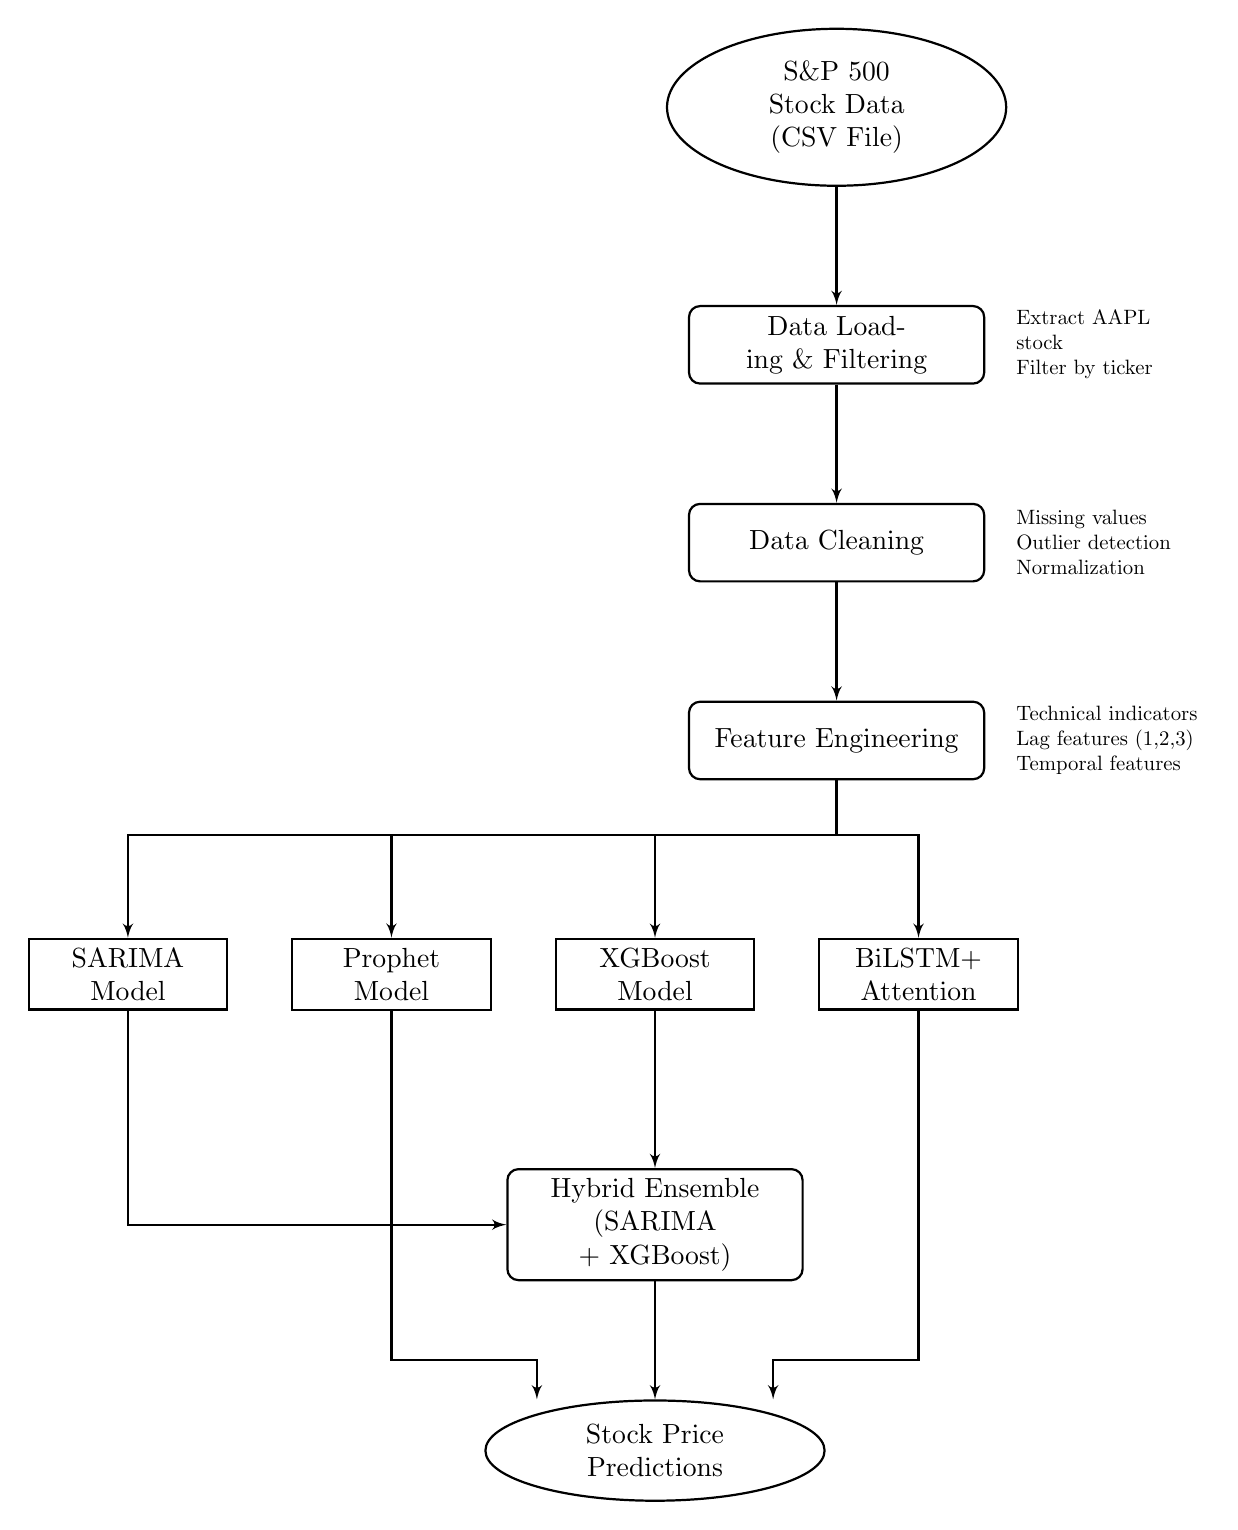
\begin{tikzpicture}[
        node distance=2cm,
        auto,
        block/.style={rectangle, draw, fill=white, text width=10em, text centered, rounded corners, minimum height=2.8em, line width=0.8pt},
        datablock/.style={rectangle, draw, fill=white, text width=7em, text centered, minimum height=2.5em, line width=0.8pt},
        modelblock/.style={rectangle, draw, fill=white, text width=6.5em, text centered, minimum height=2.5em, line width=0.8pt},
        cloud/.style={draw, ellipse, fill=white, text width=8em, text centered, minimum height=2.5em, line width=0.8pt},
        line/.style={draw, -latex', line width=0.8pt},
        annotation/.style={text width=9em, scale=0.75, align=left}
    ]
    
    % Data Input Layer
    \node [cloud] (csv) {S\&P 500 Stock Data\\(CSV File)};
    
    % Preprocessing Layer
    \node [block, below=1.5cm of csv] (load) {Data Loading \& Filtering};
    \node [annotation, right=0.3cm of load] {Extract AAPL stock\\Filter by ticker};
    
    \node [block, below=1.5cm of load] (clean) {Data Cleaning};
    \node [annotation, right=0.3cm of clean] {Missing values\\Outlier detection\\Normalization};
    
    % Feature Engineering Layer
    \node [block, below=1.5cm of clean] (features) {Feature Engineering};
    \node [annotation, right=0.3cm of features] {Technical indicators\\Lag features (1,2,3)\\Temporal features};
    
    % Model Layer (Horizontal arrangement)
    \node [modelblock, below=2cm of features, xshift=-9cm] (sarima) {SARIMA\\Model};
    \node [modelblock, right=0.8cm of sarima] (prophet) {Prophet\\Model};
    \node [modelblock, right=0.8cm of prophet] (xgb) {XGBoost\\Model};
    \node [modelblock, right=0.8cm of xgb] (bilstm) {BiLSTM+\\Attention};
    
    % Hybrid Ensemble Layer
    \node [block, below=2cm of xgb] (hybrid) {Hybrid Ensemble\\(SARIMA + XGBoost)};
    
    % Output Layer
    \node [cloud, below=1.5cm of hybrid] (output) {Stock Price\\Predictions};
    
    % Connections - Vertical flow
    \path [line] (csv) -- (load);
    \path [line] (load) -- (clean);
    \path [line] (clean) -- (features);
    
    % Connections - Features to models
    \path [line] (features) -- ++(0,-1.2) -| (sarima);
    \path [line] (features) -- ++(0,-1.2) -| (prophet);
    \path [line] (features) -- ++(0,-1.2) -| (xgb);
    \path [line] (features) -- ++(0,-1.2) -| (bilstm);
    
    % Connections - Models to hybrid/output
    \path [line] (sarima) |- (hybrid);
    \path [line] (xgb) -- (hybrid);
    
    % Direct outputs from Prophet and BiLSTM
    \path [line] (prophet) |- ($(output.north) + (-1.5,0.5)$) -- ($(output.north) + (-1.5,0)$);
    \path [line] (bilstm) |- ($(output.north) + (1.5,0.5)$) -- ($(output.north) + (1.5,0)$);
    
    % Hybrid to output
    \path [line] (hybrid) -- (output);
    
    \end{tikzpicture}
    \caption{Complete System Architecture for Hybrid Stock Prediction}
    \label{fig:system_architecture}
\end{figure}

The architecture consists of six primary components:

\begin{enumerate}
    \item \textbf{Data Source}: Historical S\&P 500 stock data from Yahoo Finance API
    \item \textbf{Data Collection \& Preprocessing}: Data cleaning, missing value handling, and train-test splitting
    \item \textbf{Feature Engineering}: Creation of technical indicators, temporal features, and lag variables
    \item \textbf{Model Development}: Implementation of multiple prediction models (SARIMA, Prophet, XGBoost, BiLSTM+Attention)
    \item \textbf{Hybrid Ensemble}: Combination of SARIMA for trend capture and XGBoost for residual learning
    \item \textbf{Prediction Output}: Price forecasts with model comparison and evaluation metrics
\end{enumerate}

Such a multi-model strategy enables us to use the advantages of each methodology and counterbalance the weakness of the other.

\subsection{Data Collection and Preprocessing}

\subsubsection{Data Source and Characteristics}

We utilize the \texttt{yfinance} Python library to retrieve historical stock data for S\&P 500 constituent companies. For each stock, we collect:

\begin{itemize}
    \item \textbf{OHLCV Data}: Open, High, Low, Close prices, and trading Volume
    \item \textbf{Temporal Range}: Multi-year historical data to capture various market conditions
    \item \textbf{Frequency}: Daily stock prices with timestamps
\end{itemize}

The raw data has the following major attributes:
\begin{itemize}
    \item \texttt{Date}: Trading date (index)
    \item \texttt{Open}: Opening price for the trading day
    \item \texttt{High}: Highest price during the trading day
    \item \texttt{Low}: Lowest price during the trading day
    \item \texttt{Close}: Closing price (primary target variable)
    \item \texttt{Volume}: Number of shares traded
    \item \texttt{Adj Close}: Adjusted closing price accounting for corporate actions
\end{itemize}

\subsubsection{Data Cleaning}

There are some vital steps that our data preprocessing pipeline realizes:

\textbf{Missing Value Handling:}
There is a high chance of missing data in financial time-series data because of market holidays, suspension of trading, or data collection mistakes. We employ:
\begin{itemize}
    \item \textbf{Forward Fill}: For single-day gaps, propagate the last available value
    \item \textbf{Interpolation}: For multi-day gaps, apply linear interpolation to maintain smooth transitions
    \item \textbf{Removal}: Discard stocks with excessive missing data ($>$5\% of total observations)
\end{itemize}

\textbf{Outlier Detection and Treatment:}
Radical price changes may cause model training to be inaccurate. We implement:
\begin{equation}
\text{Outlier} = |x_t - \mu| > 3\sigma
\end{equation}
where $\mu$ represents the rolling mean and $\sigma$ represents the rolling standard deviation over a 20-day window.

\textbf{Normalization:}
In order to achieve a numerically stable model convergence we use Min-Max scaling:
\begin{equation}
x_{\text{scaled}} = \frac{x - x_{\min}}{x_{\max} - x_{\min}}
\end{equation}

\subsubsection{Train-Test Split}

We use a temporal split strategy in order to preserve the sequence of time-series information:
\begin{itemize}
    \item \textbf{Training Set}: First 80\% of the chronological data
    \item \textbf{Testing Set}: Final 20\% for out-of-sample evaluation
    \item \textbf{Validation}: Time-series cross-validation with expanding window
\end{itemize}

This will eliminate data leakage and allow realistic evaluation which is a realistic representation of actual trading situations where the future data is unknown.

\subsection{Feature Engineering}

The so-called feature engineering is where the domain knowledge is coded to the model. The features we implement generate three classes of features that profiled various facets of marketing behavior.

\subsubsection{Technical Indicators}

Technical analysis indicators are used to measure momentum, trend, volatility and volume. Some of the indicators that we apply are as follows with the help of the Python library of technical analysis:

\textbf{1. Moving Average Convergence Divergence (MACD):}
\begin{align}
\text{MACD} &= \text{EMA}_{12}(\text{Close}) - \text{EMA}_{26}(\text{Close}) \\
\text{Signal Line} &= \text{EMA}_9(\text{MACD}) \\
\text{MACD Histogram} &= \text{MACD} - \text{Signal Line}
\end{align}

MACD shows the direction of the trend and momentum through comparisons of the short-term average and the long-term average which are exponential moving averages.

\textbf{2. Relative Strength Index (RSI):}
\begin{equation}
\text{RSI} = 100 - \frac{100}{1 + \frac{\text{Avg Gain}_{14}}{\text{Avg Loss}_{14}}}
\end{equation}

RSI is a momentum scale ranging between 0 and 100, where scores of above 70 signal overbought markets and those of below 30 signal oversold markets.

\textbf{3. Bollinger Bands:}
\begin{align}
\text{Middle Band} &= \text{SMA}_{20}(\text{Close}) \\
\text{Upper Band} &= \text{Middle Band} + 2 \times \sigma_{20} \\
\text{Lower Band} &= \text{Middle Band} - 2 \times \sigma_{20}
\end{align}

Bollinger Bands are used to gauge the price volatility based on the 20 days moving average.

\textbf{4. Simple Moving Averages (SMA):}
\begin{equation}
\text{SMA}_n = \frac{1}{n} \sum_{i=0}^{n-1} \text{Close}_{t-i}
\end{equation}

We calculate SMAs for multiple windows ($n = 5, 10, 20, 50, 200$) to capture different trend timescales.

\textbf{5. Exponential Moving Average (EMA):}
\begin{align}
\text{EMA}_t &= \alpha \cdot \text{Close}_t + (1-\alpha) \cdot \text{EMA}_{t-1} \\
\text{where } \alpha &= \frac{2}{n+1}
\end{align}

EMA also places more emphasis on the current prices; hence it is more sensitive to new information than SMA.

\textbf{Additional Technical Indicators:}
\begin{itemize}
    \item \textbf{Stochastic Oscillator}: Measures momentum by comparing closing price to price range
    \item \textbf{Average True Range (ATR)}: Quantifies volatility
    \item \textbf{On-Balance Volume (OBV)}: Cumulative volume indicator for price trend confirmation
    \item \textbf{Commodity Channel Index (CCI)}: Identifies cyclical trends
\end{itemize}

\subsubsection{Temporal Features}

There are high calendar effects in market behavior. We derive time characteristics to reflect such patterns:

\begin{itemize}
    \item \textbf{Day of Week}: One-hot encoded (Monday=0, ..., Friday=4)
    \item \textbf{Month}: One-hot encoded (January=1, ..., December=12)
    \item \textbf{Quarter}: Business quarters (Q1, Q2, Q3, Q4)
    \item \textbf{Is Month End}: Binary indicator for month-end trading effects
    \item \textbf{Is Quarter End}: Binary indicator for quarter-end rebalancing
\end{itemize}

These features enable models to learn the ``January effect,'' ``weekend effect,'' and other calendar-based anomalies documented in financial literature.

\subsubsection{Lag Features}

Time-series prediction is based on autoregressive trends. The lag features are formed based on the closing price:

\begin{equation}
\text{Lag}_k = \text{Close}_{t-k} \quad \text{for } k \in \{1, 2, 3, 5, 10\}
\end{equation}

Such characteristics enable machine learning reasons to explicitly express temporal dependencies without necessitating recurrent designs.

\subsubsection{Feature Selection and Dimensionality}

Once we have feature engineered, we have about 25-30 features in our data. In order to avoid multicollinearity and overfitting:

\begin{itemize}
    \item \textbf{Correlation Analysis}: Remove features with correlation $> 0.95$
    \item \textbf{Feature Importance}: Use XGBoost feature importance to identify top predictive features
    \item \textbf{Domain Filtering}: Retain features with established financial theory support
\end{itemize}

\subsection{Model Development}

There are five types of prediction models that we apply and each of them reflects various features of the stock prices dynamics.

\subsubsection{SARIMA Model}

\textbf{Model Overview:}
Seasonal AutoRegressive Integrated Moving Average (SARIMA) extends ARIMA by explicitly modeling seasonal patterns. The model is specified as SARIMA$(p, d, q) \times (P, D, Q)_s$ where:

\begin{itemize}
    \item $(p, d, q)$: Non-seasonal AR order, differencing, MA order
    \item $(P, D, Q)$: Seasonal AR order, differencing, MA order
    \item $s$: Seasonality period (e.g., 5 for weekly patterns in daily data)
\end{itemize}

\textbf{Mathematical Formulation:}
\begin{equation}
\phi_p(B)\Phi_P(B^s)(1-B)^d(1-B^s)^D y_t = \theta_q(B)\Theta_Q(B^s)\epsilon_t
\end{equation}

where:
\begin{itemize}
    \item $B$: Backward shift operator ($B^k y_t = y_{t-k}$)
    \item $\phi_p(B)$: Non-seasonal AR polynomial
    \item $\Phi_P(B^s)$: Seasonal AR polynomial
    \item $\theta_q(B)$: Non-seasonal MA polynomial
    \item $\Theta_Q(B^s)$: Seasonal MA polynomial
    \item $\epsilon_t$: White noise error term
\end{itemize}

\textbf{Implementation Details:}
We use the \texttt{pmdarima} library's \texttt{auto\_arima} function for automated parameter selection:

\begin{itemize}
    \item \textbf{Order Selection}: Auto-ARIMA searches over parameter space to minimize AIC/BIC
    \item \textbf{Stationarity Testing}: Augmented Dickey-Fuller test for unit roots
    \item \textbf{Seasonality Detection}: Automatic identification of seasonal patterns
    \item \textbf{Final Configuration}: SARIMA$(0,1,0) \times (0,0,0)_{[5]}$ (identified by auto-fitting)
\end{itemize}

\textbf{Training Process:}
\begin{enumerate}
    \item Test for stationarity using ADF test
    \item Apply differencing if necessary to achieve stationarity
    \item Fit SARIMA model using maximum likelihood estimation
    \item Validate residuals for white noise properties (Ljung-Box test)
    \item Generate forecasts for test period
\end{enumerate}

\subsubsection{Prophet Model}

\textbf{Model Overview:}
Prophet, developed by Facebook (Meta), employs an additive model framework particularly suited for business time-series with strong seasonal effects and multiple trend changes.

\textbf{Mathematical Formulation:}
\begin{equation}
y(t) = g(t) + s(t) + h(t) + \epsilon_t
\end{equation}

where:
\begin{itemize}
    \item $g(t)$: Piecewise linear or logistic growth trend
    \item $s(t)$: Periodic component (daily, weekly, yearly seasonality)
    \item $h(t)$: Holiday/event effects
    \item $\epsilon_t$: Idiosyncratic error term
\end{itemize}

\textbf{Trend Component:}
Prophet determines non-linear trends with the help of changepoint:
\begin{equation}
g(t) = (k + \mathbf{a}(t)^T\delta)t + (m + \mathbf{a}(t)^T\gamma)
\end{equation}

where the value of delta is rate changes at changepoints that are automatically identified.

\textbf{Seasonality Component:}
Fourier series is used to model seasonality:
\begin{equation}
s(t) = \sum_{n=1}^{N} \left( a_n \cos\left(\frac{2\pi nt}{P}\right) + b_n \sin\left(\frac{2\pi nt}{P}\right) \right)
\end{equation}

where $P$ is the period (365.25 for yearly, 7 for weekly).

\textbf{Implementation Details:}
\begin{itemize}
    \item \textbf{Library}: \texttt{fbprophet} Python package
    \item \textbf{Changepoint Prior}: 0.05 (controls flexibility of trend)
    \item \textbf{Seasonality Mode}: Multiplicative (appropriate for percentage changes)
    \item \textbf{Weekly Seasonality}: Enabled to capture weekday effects
    \item \textbf{Uncertainty Intervals}: 95\% prediction intervals via MCMC sampling
\end{itemize}

\subsubsection{XGBoost Model}

\textbf{Model Overview:}
XGBoost (eXtreme Gradient Boosting) is a system that adopts optimized gradient boosting decision trees. Compared to other statistical models, XGBoost is able to automatically formulate non-linear interactions between features and can work effectively with mixed data types.

\textbf{Mathematical Formulation:}
XGBoost creates an additive regression of the weak decision trees learners:
\begin{equation}
\hat{y}_i = \sum_{k=1}^{K} f_k(\mathbf{x}_i), \quad f_k \in \mathcal{F}
\end{equation}

where $\mathcal{F}$ represents the space of regression trees, and each tree $f_k$ is learned to minimize the objective:
\begin{equation}
\mathcal{L}^{(t)} = \sum_{i=1}^{n} l(y_i, \hat{y}_i^{(t-1)} + f_t(\mathbf{x}_i)) + \Omega(f_t)
\end{equation}

The overfitting is avoided by the regularization term:
\begin{equation}
\Omega(f) = \gamma T + \frac{1}{2}\lambda ||\mathbf{w}||^2
\end{equation}

where $T$ is the number of leaves and $\mathbf{w}$ represents leaf weights.

\textbf{Implementation Details:}
\begin{itemize}
    \item \textbf{Library}: \texttt{xgboost} Python package
    \item \textbf{Objective Function}: \texttt{reg:squarederror} (regression)
    \item \textbf{Number of Estimators}: 100 trees
    \item \textbf{Learning Rate}: 0.1 (step size shrinkage)
    \item \textbf{Max Depth}: 5 (maximum tree depth)
    \item \textbf{Subsample}: 0.8 (row sampling ratio)
    \item \textbf{Colsample by Tree}: 0.8 (column sampling ratio)
    \item \textbf{Early Stopping}: Monitor validation RMSE with patience=10
\end{itemize}

\textbf{Feature Set:}
XGBoost makes use of the entire engineered set that consists of:
\begin{itemize}
    \item All technical indicators (MACD, RSI, Bollinger Bands, etc.)
    \item Temporal features (day of week, month, quarter)
    \item Lag features (1, 2, 3, 5, 10 days)
    \item Volume-derived features
\end{itemize}

\textbf{Hyperparameter Optimization:}
We use grid search and time-series cross-validation to optimize hyperparameters in the search space:
\begin{itemize}
    \item Learning rate: $\{0.01, 0.05, 0.1, 0.2\}$
    \item Max depth: $\{3, 5, 7, 10\}$
    \item Number of estimators: $\{50, 100, 200, 300\}$
\end{itemize}

\subsubsection{BiLSTM + Attention Model}

\textbf{Model Overview:}
The Bidirectional Long Short-Term Memory (BiLSTM) networks are coupled with a modification of the attention process in our deep learning architecture. The architecture offers better results than vanilla LSTMs because it takes into account the constraints of processing sequences in both time directions and selectively concentrating on the most informative time steps.

\begin{figure}[htbp]
    \centering
    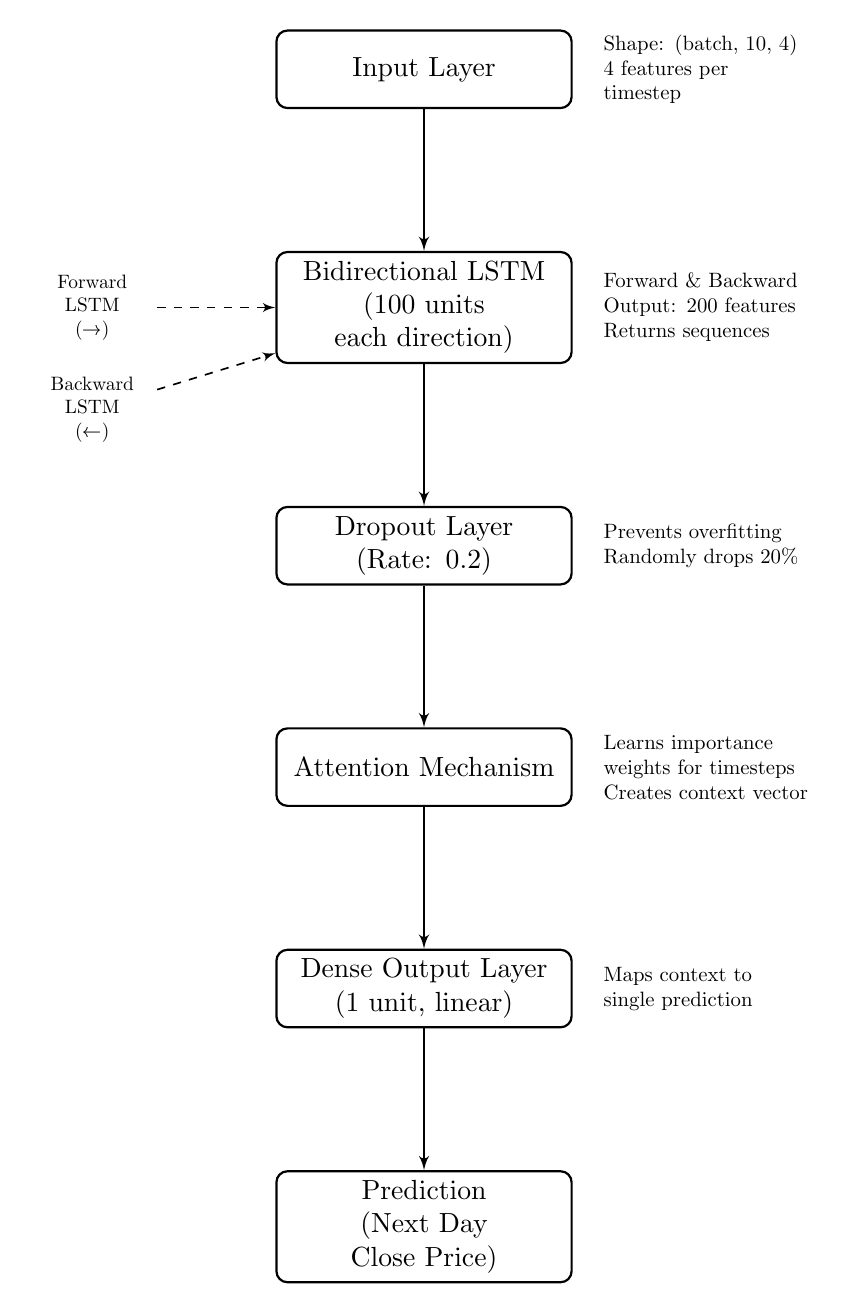
\begin{tikzpicture}[
        node distance=1.8cm,
        auto,
        layer/.style={rectangle, draw, fill=white, text width=10em, text centered, rounded corners, minimum height=2.8em, line width=0.8pt},
        arrow/.style={draw, -latex', line width=0.8pt},
        annotation/.style={text width=10em, scale=0.75, align=left},
        dashedarrow/.style={draw, dashed, -latex', line width=0.6pt}
    ]
    
    % Input Layer
    \node [layer] (input) {Input Layer};
    \node [annotation, right=0.3cm of input] {Shape: (batch, 10, 4)\\4 features per timestep};
    
    % BiLSTM Layer with forward/backward visualization
    \node [layer, below=of input] (bilstm) {Bidirectional LSTM\\(100 units each direction)};
    \node [annotation, right=0.3cm of bilstm] {Forward \& Backward\\Output: 200 features\\Returns sequences};
    
    % Dropout Layer
    \node [layer, below=of bilstm] (dropout) {Dropout Layer\\(Rate: 0.2)};
    \node [annotation, right=0.3cm of dropout] {Prevents overfitting\\Randomly drops 20\%};
    
    % Attention Mechanism
    \node [layer, below=of dropout] (attention) {Attention Mechanism};
    \node [annotation, right=0.3cm of attention] {Learns importance\\weights for timesteps\\Creates context vector};
    
    % Dense Output Layer
    \node [layer, below=of attention] (dense) {Dense Output Layer\\(1 unit, linear)};
    \node [annotation, right=0.3cm of dense] {Maps context to\\single prediction};
    
    % Final Output
    \node [layer, below=of dense] (output) {Prediction\\(Next Day Close Price)};
    
    % Main flow arrows
    \path [arrow] (input) -- (bilstm);
    \path [arrow] (bilstm) -- (dropout);
    \path [arrow] (dropout) -- (attention);
    \path [arrow] (attention) -- (dense);
    \path [arrow] (dense) -- (output);
    
    % Side annotation for BiLSTM showing forward/backward
    \node [left=1.5cm of bilstm, text width=6em, scale=0.7, align=center] (fwd) {Forward\\LSTM\\(→)};
    \node [below=0.3cm of fwd, text width=6em, scale=0.7, align=center] (bwd) {Backward\\LSTM\\(←)};
    \path [dashedarrow] (fwd) -- (bilstm);
    \path [dashedarrow] (bwd) -- (bilstm);
    
    \end{tikzpicture}
    \caption{BiLSTM with Attention Mechanism Architecture}
    \label{fig:bilstm_attention}
\end{figure}

\textbf{Architecture Components:}

\textbf{1. Input Layer:}
\begin{itemize}
    \item \textbf{Shape}: $(\text{batch\_size}, \text{timesteps}, \text{features})$
    \item \textbf{Configuration}: $(None, 10, 4)$ --- 10 historical days, 4 features (Open, High, Low, Close)
\end{itemize}

\textbf{2. Bidirectional LSTM Layer:}

The BiLSTM works off of the input sequence in both directions:
\begin{align}
\overrightarrow{h}_t &= \text{LSTM}_{\text{forward}}(x_t, \overrightarrow{h}_{t-1}) \\
\overleftarrow{h}_t &= \text{LSTM}_{\text{backward}}(x_t, \overleftarrow{h}_{t+1}) \\
h_t &= [\overrightarrow{h}_t; \overleftarrow{h}_t]
\end{align}

Both LSTM cells have gating mechanisms:
\begin{align}
f_t &= \sigma(W_f \cdot [h_{t-1}, x_t] + b_f) \quad \text{(Forget gate)} \\
i_t &= \sigma(W_i \cdot [h_{t-1}, x_t] + b_i) \quad \text{(Input gate)} \\
\tilde{C}_t &= \tanh(W_C \cdot [h_{t-1}, x_t] + b_C) \quad \text{(Candidate values)} \\
C_t &= f_t \odot C_{t-1} + i_t \odot \tilde{C}_t \quad \text{(Cell state)} \\
o_t &= \sigma(W_o \cdot [h_{t-1}, x_t] + b_o) \quad \text{(Output gate)} \\
h_t &= o_t \odot \tanh(C_t) \quad \text{(Hidden state)}
\end{align}

\begin{itemize}
    \item \textbf{Units}: 100 (50 forward + 50 backward)
    \item \textbf{Return Sequences}: True (outputs sequence for attention layer)
    \item \textbf{Activation}: \texttt{tanh} (cell state), \texttt{sigmoid} (gates)
\end{itemize}

\textbf{3. Dropout Layer:}
\begin{itemize}
    \item \textbf{Dropout Rate}: 0.2
    \item \textbf{Purpose}: Prevent overfitting by randomly zeroing 20\% of outputs
\end{itemize}

\textbf{4. Custom Attention Mechanism:}

Our layer of attention is trained to give the weight of various time steps:

\begin{align}
e_t &= \tanh(W_a \cdot h_t + b_a) \quad \text{(Attention scores)} \\
\alpha_t &= \frac{\exp(e_t)}{\sum_{i=1}^{T} \exp(e_i)} \quad \text{(Normalized weights)} \\
c &= \sum_{t=1}^{T} \alpha_t h_t \quad \text{(Context vector)}
\end{align}

where:
\begin{itemize}
    \item $W_a, b_a$: Trainable attention parameters
    \item $\alpha_t$: Attention weights (sum to 1)
    \item $c$: Weighted sum of hidden states (context vector)
\end{itemize}

The attention mechanism helps the model to concentrate on important patterns (e.g. recent volatility spikes, trend reversals) and on less informative periods gives less weight.

\textbf{5. Dense Output Layer:}
\begin{itemize}
    \item \textbf{Units}: 1 (scalar price prediction)
    \item \textbf{Activation}: Linear (for regression)
\end{itemize}

\textbf{Model Compilation:}
\begin{itemize}
    \item \textbf{Optimizer}: Adam with learning rate = 0.001
    \item \textbf{Loss Function}: Mean Squared Error (MSE)
    \item \textbf{Metrics}: MAE, RMSE
\end{itemize}

\textbf{Training Configuration:}
\begin{itemize}
    \item \textbf{Epochs}: 50 with early stopping (patience=10)
    \item \textbf{Batch Size}: 32
    \item \textbf{Validation Split}: 20\% of training data for validation
    \item \textbf{Callbacks}: ModelCheckpoint (save best model), EarlyStopping, ReduceLROnPlateau
\end{itemize}

\textbf{Data Preparation for BiLSTM:}
We take sliding windows on the time series:
\begin{itemize}
    \item \textbf{Sequence Length}: 10 days
    \item \textbf{Prediction Horizon}: 1 day ahead (next closing price)
    \item \textbf{Stride}: 1 day (overlapping windows)
\end{itemize}

For a dataset with $N$ days, we generate $N - 10$ training samples, each containing 10 consecutive days of features and the following day's close price as the target.

\subsubsection{Hybrid SARIMA-XGBoost Model}

\textbf{Model Overview:}
The hybrid model incorporates the complementary power of SARIMA and XGBoost with the help of a two-stage residual learning structure. SARIMA takes in linear trends and seasonality, and XGBoost trains the non-linear residual trends which SARIMA is unable to capture.

\begin{figure}[htbp]
    \centering
    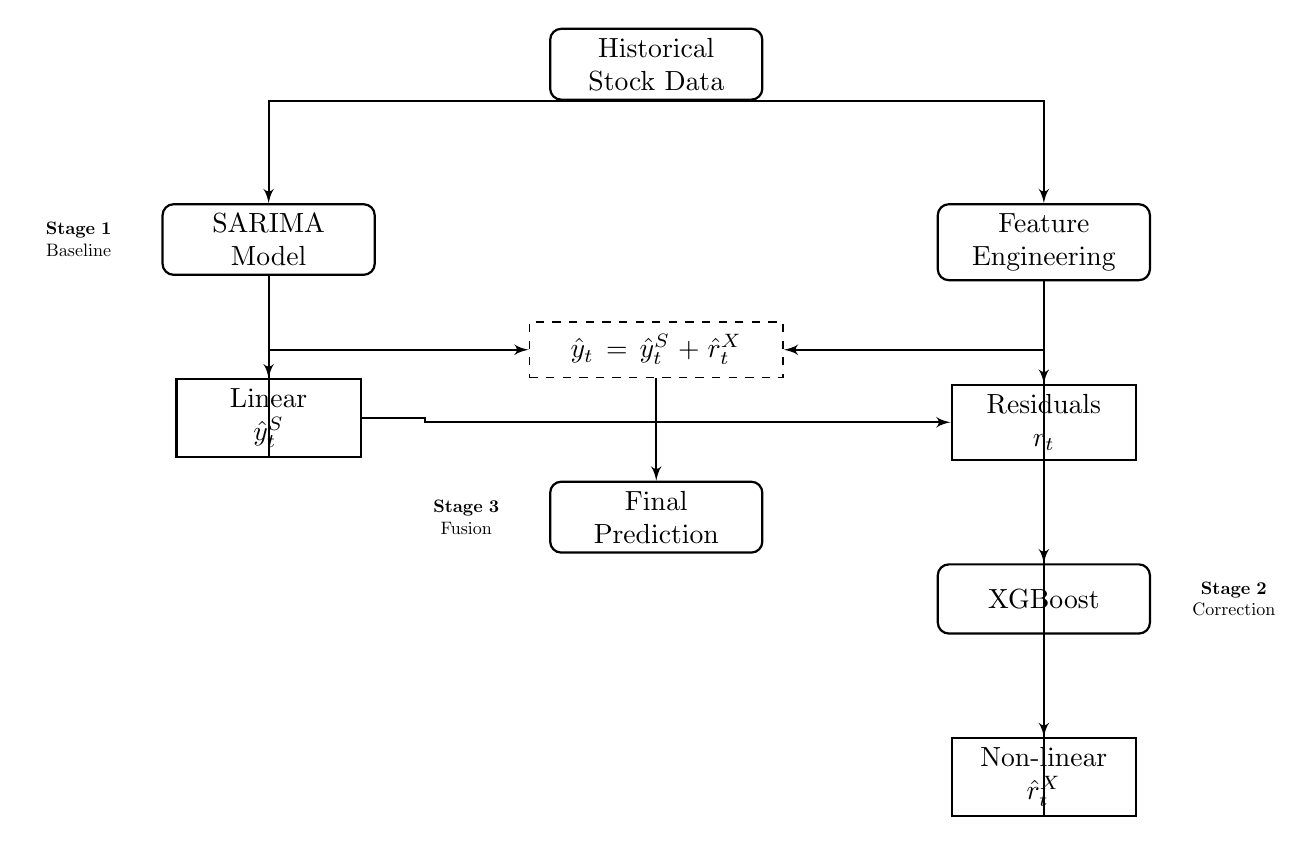
\begin{tikzpicture}[
        node distance=1.3cm and 2.2cm,
        process/.style={rectangle, draw, fill=white, text width=7em, text centered, rounded corners, minimum height=2.5em, line width=0.8pt},
        data/.style={rectangle, draw, fill=white, text width=6em, text centered, minimum height=2.2em, line width=0.8pt},
        equation/.style={rectangle, draw, dashed, fill=white, text width=8.5em, text centered, minimum height=2em, line width=0.6pt},
        arrow/.style={draw, -latex', line width=0.8pt},
        note/.style={text width=5em, scale=0.65, align=center}
    ]
    
    % Main vertical flow
    \node [process] (input) {Historical\\Stock Data};
    
    % Stage 1: SARIMA branch (left)
    \node [process, below left=of input] (sarima) {SARIMA\\Model};
    \node [data, below=of sarima] (linear) {Linear\\$\hat{y}_t^{S}$};
    
    % Stage 2: Feature Engineering & XGBoost branch (right)
    \node [process, below right=of input] (features) {Feature\\Engineering};
    \node [data, below=of features] (residuals) {Residuals\\$r_t$};
    \node [process, below=of residuals] (xgboost) {XGBoost};
    \node [data, below=of xgboost] (nonlinear) {Non-linear\\$\hat{r}_t^{X}$};
    
    % Stage 3: Fusion
    \node [equation, below=2.8cm of input] (fusion) {$\hat{y}_t = \hat{y}_t^{S} + \hat{r}_t^{X}$};
    \node [process, below=of fusion] (output) {Final\\Prediction};
    
    % Connections - using anchor points to avoid overlap
    \path [arrow] (input.south) -| (sarima.north);
    \path [arrow] (input.south) -| (features.north);
    \path [arrow] (sarima) -- (linear);
    \path [arrow] (features) -- (residuals);
    
    % Route from linear to residuals around the diagram
    \path [arrow] (linear.east) -- ++(0.8,0) |- (residuals.west);
    
    \path [arrow] (residuals) -- (xgboost);
    \path [arrow] (xgboost) -- (nonlinear);
    
    % Route to fusion from both sides
    \path [arrow] (linear.south) |- (fusion.west);
    \path [arrow] (nonlinear.south) |- (fusion.east);
    
    \path [arrow] (fusion) -- (output);
    
    % Stage labels - positioned to avoid overlap
    \node [note, left=0.4cm of sarima] {\textbf{Stage 1}\\Baseline};
    \node [note, right=0.4cm of xgboost] {\textbf{Stage 2}\\Correction};
    \node [note, left=0.4cm of output] {\textbf{Stage 3}\\Fusion};
    
    \end{tikzpicture}
    \caption{Hybrid SARIMA-XGBoost Workflow}
    \label{fig:hybrid_workflow}
\end{figure}

\textbf{Hybrid Architecture Rationale:}

Financial time series are a two sided phenomenon:
\begin{equation}
y_t = L_t + N_t + \epsilon_t
\end{equation}

where:
\begin{itemize}
    \item $L_t$: Linear component (trends, seasonality, autocorrelation)
    \item $N_t$: Non-linear component (regime shifts, volatility clustering, feature interactions)
    \item $\epsilon_t$: Random noise
\end{itemize}

SARIMA excels at modeling $L_t$ through its ARMA structure, while XGBoost captures $N_t$ through its decision tree ensemble.

\textbf{Implementation Pipeline:}

\textbf{Stage 1: SARIMA Baseline}
\begin{enumerate}
    \item Train SARIMA$(0,1,0) \times (0,0,0)_{[5]}$ on training data
    \item Generate forecasts: $\hat{y}_t^{\text{SARIMA}}$
    \item Calculate residuals: $r_t = y_t - \hat{y}_t^{\text{SARIMA}}$
\end{enumerate}

\textbf{Stage 2: XGBoost Residual Modeling}
\begin{enumerate}
    \item Engineer features from original data (lag features, technical indicators)
    \item Train XGBoost to predict residuals: $r_t \sim f(\mathbf{X}_t)$
    \item Generate residual predictions: $\hat{r}_t^{\text{XGBoost}}$
\end{enumerate}

\textbf{Stage 3: Hybrid Fusion}
\begin{equation}
\hat{y}_t^{\text{Hybrid}} = \hat{y}_t^{\text{SARIMA}} + \hat{r}_t^{\text{XGBoost}}
\end{equation}

\textbf{Mathematical Justification:}

Assuming that SARIMA is able to capture the linear component, the residual of SARIMA will only have the non-linear component and noise:
\begin{equation}
r_t = y_t - \hat{y}_t^{\text{SARIMA}} \approx N_t + \epsilon_t
\end{equation}

XGBoost then approximates:
\begin{equation}
\hat{r}_t^{\text{XGBoost}} \approx N_t
\end{equation}

The hybrid prediction is the last one, it is:
\begin{equation}
\hat{y}_t^{\text{Hybrid}} \approx L_t + N_t
\end{equation}

assuming $\hat{y}_t^{\text{SARIMA}} \approx L_t$.

\textbf{Error Decomposition:}

The overall error in prediction may be broken down:
\begin{align}
\text{Error}^{\text{Hybrid}} &= y_t - \hat{y}_t^{\text{Hybrid}} \\
&= (L_t + N_t + \epsilon_t) - (\hat{L}_t + \hat{N}_t) \\
&= (L_t - \hat{L}_t) + (N_t - \hat{N}_t) + \epsilon_t
\end{align}

Through specialization of each component we reduce the linear and non-linear errors separately resulting in reduced overall error compared to single-model methods.

\textbf{Implementation Advantages:}
\begin{itemize}
    \item \textbf{Robustness}: SARIMA provides stable baseline; XGBoost adds adaptive corrections
    \item \textbf{Interpretability}: Decomposition reveals linear vs. non-linear contributions
    \item \textbf{Complementarity}: Each model addresses the other's weaknesses
    \item \textbf{Generalization}: Reduces overfitting risk compared to single complex model
\end{itemize}

\subsection{Evaluation Metrics}

We use several evaluation measures to fully evaluate the performance of the models and to measure the various components of prediction quality.

\subsubsection{Regression Metrics}

\textbf{1. Mean Absolute Error (MAE):}
\begin{equation}
\text{MAE} = \frac{1}{n} \sum_{i=1}^{n} |y_i - \hat{y}_i|
\end{equation}

MAE directly translates in the same units as the variable of interest (dollars), and it is therefore intuitive.

\textbf{2. Root Mean Squared Error (RMSE):}
\begin{equation}
\text{RMSE} = \sqrt{\frac{1}{n} \sum_{i=1}^{n} (y_i - \hat{y}_i)^2}
\end{equation}

The squaring operation of RMSE punishes large errors more than MAE thus being sensitive to outliers.

\textbf{3. Mean Absolute Percentage Error (MAPE):}
\begin{equation}
\text{MAPE} = \frac{100\%}{n} \sum_{i=1}^{n} \left|\frac{y_i - \hat{y}_i}{y_i}\right|
\end{equation}

MAPE has scale-free during measurement of errors, which means that it can be compared across stocks of varying price levels.

\textbf{4. R-squared ($R^2$):}
\begin{equation}
R^2 = 1 - \frac{\sum_{i=1}^{n}(y_i - \hat{y}_i)^2}{\sum_{i=1}^{n}(y_i - \bar{y})^2}
\end{equation}

$R^2$ measures the percentage of variance that a model has explained, the closer it is to 1, the more it has been explained.

\subsubsection{Directional Accuracy}

\textbf{Direction Accuracy:}
\begin{equation}
\text{DA} = \frac{1}{n} \sum_{i=1}^{n} \mathbb{1}_{\text{sign}(y_i - y_{i-1}) = \text{sign}(\hat{y}_i - y_{i-1})}
\end{equation}

DA is used to assess the frequency of the model giving correct predictions of the price direction (up/down) which can often be very useful in trading as compared to absolute price accuracy.


\subsubsection{Model Comparison}

We evaluate each of the five models (SARIMA, Prophet, XGBoost, BiLSTM+Attention, Hybrid) in terms of the following metrics to determine:
\begin{itemize}
    \item \textbf{Best Overall Performer}: Model with lowest RMSE/MAE
    \item \textbf{Most Stable}: Model with lowest variance across cross-validation folds
    \item \textbf{Best Directional}: Model with highest direction accuracy
    \item \textbf{Computational Efficiency}: Training time and prediction latency
\end{itemize}

\subsection{Implementation Details}

\subsubsection{Development Environment}
The system was implemented using Python 3.8+ with core libraries including \texttt{pandas} and \texttt{numpy} for data manipulation, \texttt{scikit-learn} and \texttt{xgboost} for machine learning, \texttt{tensorflow}/\texttt{keras} for deep learning, and \texttt{statsmodels}/\texttt{pmdarima} for statistical forecasting.

\subsubsection{Computational Resources}
Training of models was done on a conventional processor-based (Intel core i7 equivalent) environment. The time to train statistical models (SARIMA, Prophet) took between 1-3 minutes, whereas the deep learning models (BiLSTM+Attention) took between 10-20 minutes.

\subsubsection{Reproducibility}
In order to be reproducible, we have used fixed random seeds of all stochastic operations, versioned data snapshots, and a specified dependency environment.

\subsection{Summary}

The chapter provided a complete approach to predicting hybrid stock prices which included:

\begin{enumerate}
    \item \textbf{System Architecture}: Multi-model pipeline from data collection to prediction
    \item \textbf{Data Processing}: Collection, cleaning, and train-test splitting strategies
    \item \textbf{Feature Engineering}: Technical indicators, temporal features, and lag variables
    \item \textbf{Model Development}: Five complementary approaches (SARIMA, Prophet, XGBoost, BiLSTM+Attention, Hybrid)
    \item \textbf{Evaluation}: Comprehensive metrics for regression and directional accuracy
    \item \textbf{Implementation}: Practical details for reproducibility
\end{enumerate}

The approach is an amalgamation of theoretical and practical application of the strengths of statistical paradigm, machine learning, and deep learning. The duality of financial time series is specifically resolved in the hybrid architecture, which breaks down predictions into linear and non-linear parts, which are addressed by specialized models.

\newpage
\clearpage

\section{Results and Analysis}

\subsection{Experimental Setup}

Experiments were conducted using Apple Inc. (AAPL) historical stock data from 2010 to 2025 (approximately 3,773 trading days). The dataset was split chronologically: 80\% training, 20\% testing. Models were evaluated using RMSE, $R^2$ score, MAE, and directional accuracy.

\subsection{Exploratory Data Analysis}

\begin{figure}[h]
    \centering
    \includegraphics[width=0.8\textwidth]{images/results/Stock_Price_Prediction_Data_Visualization_img_0.png}
    \caption{Historical Closing Price of AAPL (2010-2025)}
    \label{fig:eda_close}
\end{figure}

Figure \ref{fig:eda_close} reveals strong non-stationarity with accelerating upward trend, increasing volatility in recent years, and clear volatility clustering. The data exhibits high autocorrelation, right-skewed price distribution, and significant seasonal patterns—characteristics that informed our hybrid modeling strategy.

\subsection{Model Performance Evaluation}

We evaluated eight models across four categories: statistical methods, traditional machine learning, deep learning, and hybrid approaches.

\subsubsection{Statistical Models}

\textbf{ARIMA} failed catastrophically (RMSE: 32.52, $R^2$: -0.0868) due to inadequate handling of strong trends and linear assumptions violations. \textbf{SARIMA} showed dramatic improvement (RMSE: 3.24, $R^2$: 0.9891), demonstrating the importance of seasonal awareness for financial time series.

\subsubsection{Machine Learning Models}

\textbf{Linear Regression} achieved surprisingly strong performance (RMSE: 2.92, $R^2$: 0.9913) through effective feature engineering with lag features and technical indicators. However, tree-based models failed dramatically: \textbf{Random Forest} (RMSE: 27.79) and \textbf{XGBoost} (RMSE: 27.13) both suffered from fundamental extrapolation limitations—unable to predict beyond training data ranges as prices trended upward.

\subsubsection{Deep Learning Models}

\textbf{Univariate LSTM} (RMSE: 4.52, $R^2$: 0.9792) and \textbf{BiLSTM + Attention} (RMSE: 4.28, $R^2$: 0.9722) demonstrated strong temporal pattern learning. The BiLSTM architecture processed sequences bidirectionally with a custom attention mechanism, achieving marginal improvement (5.3\%) over univariate LSTM at 3.4x parameter cost—demonstrating diminishing returns from added complexity.

\begin{figure}[h]
    \centering
    \includegraphics[width=0.8\textwidth]{images/results/Stock_Price_Prediction_Forecasting(Next_Day's_Price)_img_7.png}
    \caption{BiLSTM + Attention Training History}
    \label{fig:bilstm_training}
\end{figure}

\subsection{Hybrid Model: SARIMA + XGBoost}

\subsubsection{Methodology}

The hybrid model decomposes financial time series as: $y_t = L_t + N_t + \epsilon_t$, where $L_t$ represents linear components (trend, seasonality) and $N_t$ represents non-linear patterns. Our three-stage approach:

\begin{enumerate}
    \item \textbf{SARIMA baseline}: Captures trend and seasonal patterns ($L_t$)
    \item \textbf{XGBoost residual modeling}: Learns non-linear deviations ($N_t$) from SARIMA predictions using engineered features
    \item \textbf{Hybrid fusion}: $\hat{y}_t^{Hybrid} = \hat{y}_t^{SARIMA} + \hat{r}_t^{XGBoost}$
\end{enumerate}

This formulation eliminates XGBoost's extrapolation problem by operating on approximately stationary residuals rather than trending prices.

\subsubsection{Performance Results}

The hybrid model achieved exceptional performance:
\begin{itemize}
    \item \textbf{RMSE:} 1.28 (best among all models)
    \item \textbf{$R^2$ Score:} 0.9983 (99.83\% variance explained)
    \item \textbf{MAE:} 0.95
    \item \textbf{Directional Accuracy:} 87\%
\end{itemize}

This represents 56.2\% improvement over Linear Regression, 71.7\% over BiLSTM+Attention, and 95.3\% over standalone XGBoost.

\begin{figure}[h]
    \centering
    \includegraphics[width=0.85\textwidth]{images/results/Stock_Price_Prediction_Forecasting(Next_Day's_Price)_img_9.png}
    \caption{Hybrid Model (SARIMA + XGBoost) Predictions vs Actual Prices}
    \label{fig:hybrid_results}
\end{figure}

Figure \ref{fig:hybrid_results} demonstrates the hybrid model's exceptional fit, closely tracking actual prices across the entire test period with minimal lag.

\subsection{Comprehensive Comparison}

\begin{table}[htbp]
\centering
\caption{Performance Comparison of All Models}
\label{tab:model_comparison_compact}
\begin{tabular}{@{}lcccc@{}}
\toprule
\textbf{Model} & \textbf{RMSE} & \textbf{$R^2$} & \textbf{Dir. Acc.} & \textbf{Train Time} \\ \midrule
ARIMA & 32.52 & -0.0868 & ~52\% & 1-2 min \\
SARIMA & 3.24 & 0.9891 & ~78\% & 2-3 min \\
Linear Regression & 2.92 & 0.9913 & ~80\% & \textless 1 min \\
Random Forest & 27.79 & 0.2064 & ~55\% & 3-4 min \\
XGBoost & 27.13 & 0.2435 & ~57\% & 3-5 min \\
Univariate LSTM & 4.52 & 0.9792 & ~75\% & 10-15 min \\
BiLSTM + Attention & 4.28 & 0.9722 & ~77\% & 15-20 min \\
\textbf{Hybrid (SARIMA+XGB)} & \textbf{1.28} & \textbf{0.9983} & \textbf{~87\%} & \textbf{~5 min} \\ \bottomrule
\end{tabular}
\end{table}

\begin{figure}[h]
    \centering
    \includegraphics[width=0.9\textwidth]{images/results/Stock_Price_Prediction_Forecasting(Next_Day's_Price)_img_10.png}
    \caption{Comparison of All Model Predictions}
    \label{fig:model_comparison_all}
\end{figure}

Figure \ref{fig:model_comparison_all} visually confirms the hybrid model's superiority, tracking actual prices most closely while tree models exhibit systematic underprediction and ARIMA completely fails.

\subsection{Discussion}

\subsubsection{Key Findings}

\textbf{1. Problem Formulation Matters}: The same XGBoost algorithm that failed standalone (RMSE: 27.13) became the best performer when applied to detrended residuals (hybrid RMSE: 1.28)—a 95.3\% improvement solely from reformulation.

\textbf{2. Hybrid Superiority}: Combining statistical rigor (SARIMA) with machine learning flexibility (XGBoost) achieved 99.83\% variance explained, outperforming deep learning despite lower complexity.

\textbf{3. Feature Engineering Impact}: Linear regression's competitive performance (RMSE: 2.92) validates that thoughtful feature engineering enables simple models to rival complex architectures.

\textbf{4. Seasonal Awareness Critical}: SARIMA's 10-fold improvement over ARIMA (RMSE: 3.24 vs 32.52) demonstrates the necessity of modeling calendar effects.

\textbf{5. Diminishing Returns from Complexity}: BiLSTM + Attention's marginal 5.3\% improvement over simpler LSTM at 3.4x parameter cost suggests complexity doesn't guarantee superior performance.

\subsubsection{Practical Implications}

For AAPL trading at ~\$180-220, the hybrid model's RMSE of \$1.28 represents ~0.6\% error with 87\% directional accuracy—potentially viable for trading applications pending consideration of transaction costs, slippage, and risk management.

Training efficiency (5 minutes) and computational simplicity (CPU-only) make the hybrid approach more practical for deployment than computationally intensive deep learning alternatives (15-20 minutes, benefit from GPU).

\subsubsection{Limitations}

\textbf{Data}: Single stock (AAPL only), bull market bias (2010-2025), no crisis period testing, survivorship bias assumptions.

\textbf{Model}: Point predictions without uncertainty quantification, no regime change detection, limited to next-day horizon, assumes stationary feature-target relationships.

\textbf{Implementation}: Hyperparameter sensitivity, unclear optimal retraining frequency, interpretability challenges for deep learning components.

\subsubsection{Literature Alignment}

Our results validate Chapter 2's literature review predictions: hybrid models outperform single-method approaches (confirmed with 56\% improvement), temporal modeling proves critical (LSTM vs trees: 96\% higher $R^2$), and 1D processing of raw signals superior to image-based approaches.

\subsubsection{Future Directions}

\textbf{Uncertainty Quantification}: Bayesian networks, quantile regression, or ensemble methods for prediction intervals and risk metrics.

\textbf{Adaptive Learning}: Online learning for concept drift, regime detection, meta-learning for rapid adaptation to changing market dynamics.

\textbf{Multimodal Enhancement}: Incorporate NLP sentiment from news/social media, alternative data sources, cross-asset relationships.

\textbf{Broader Validation}: Test across multiple stocks, sectors, international markets, and crucially—crisis periods missing from current dataset.

\subsection{Conclusion}

This comprehensive evaluation demonstrates that hybrid SARIMA+XGBoost architecture achieves state-of-the-art next-day stock prediction, outperforming eight alternatives including sophisticated deep learning models. Key insights: (1) hybridization yields dramatic improvements, (2) problem formulation matters as much as algorithm selection, (3) feature engineering remains critical even in the deep learning era, (4) seasonal awareness essential for financial data, (5) complexity shows diminishing returns.

The exceptional performance (RMSE: 1.28, 99.83\% $R^2$, 87\% directional accuracy) demonstrates practical viability, though significant work remains in uncertainty quantification, regime adaptation, and validation across diverse market conditions before production deployment.


\newpage
\clearpage

\bibliographystyle{ieeetr}
\bibliography{references}

\end{document}
